%===============================================================================
% LaTeX sjabloon voor de bachelorproef toegepaste informatica aan HOGENT
% Meer info op https://github.com/HoGentTIN/latex-hogent-report
%===============================================================================

\documentclass[dutch,dit,thesis]{hogentreport}

% TODO:
% - If necessary, replace the option `dit`' with your own department!
%   Valid entries are dbo, dbt, dgz, dit, dlo, dog, dsa, soa
% - If you write your thesis in English (remark: only possible after getting
%   explicit approval!), remove the option "dutch," or replace with "english".

\usepackage{lipsum} % For blind text, can be removed after adding actual content

%% Pictures to include in the text can be put in the graphics/ folder
\graphicspath{{graphics/}}

%% For source code highlighting, requires pygments to be installed
%% Compile with the -shell-escape flag!
\usepackage[section]{minted}
\usemintedstyle{solarized-light}
\definecolor{bg}{RGB}{253,246,227} %% Set the background color of the codeframe

%% Change this line to edit the line numbering style:
\renewcommand{\theFancyVerbLine}{\ttfamily\scriptsize\arabic{FancyVerbLine}}

%% Macro definition to load external java source files with \javacode{filename}:
\newmintedfile[javacode]{java}{
    bgcolor=bg,
    fontfamily=tt,
    linenos=true,
    numberblanklines=true,
    numbersep=5pt,
    gobble=0,
    framesep=2mm,
    funcnamehighlighting=true,
    tabsize=4,
    obeytabs=false,
    breaklines=true,
    mathescape=false
    samepage=false,
    showspaces=false,
    showtabs =false,
    texcl=false,
}

% Other packages not already included can be imported here
\usepackage{listings}
%%---------- Document metadata -------------------------------------------------
% TODO: Replace this with your own information
\author{Ruben Schrurs}
\supervisor{Dhr. T. Antjon}
\cosupervisor{Dhr. K. Dewaegenaere }
\title%
    {Ontdekken van de voordelen en beperkingen bij de implementatie van 3D-interactie in e-commerce: Een vergelijkende studie en proof-of-concept.}
\academicyear{\advance\year by -1 \the\year--\advance\year by 1 \the\year}
\examperiod{2}
\degreesought{\IfLanguageName{dutch}{Professionele bachelor in de toegepaste informatica}{Bachelor of applied computer science}}
\partialthesis{false} %% To display 'in partial fulfilment'
%\institution{Internshipcompany BVBA.}

%% Add global exceptions to the hyphenation here
\hyphenation{back-slash}

%% The bibliography (style and settings are  found in hogentthesis.cls)
\addbibresource{bachproef.bib}            %% Bibliography file
\addbibresource{../voorstel/voorstel.bib} %% Bibliography research proposal
\defbibheading{bibempty}{}

%% Prevent empty pages for right-handed chapter starts in twoside mode
\renewcommand{\cleardoublepage}{\clearpage}

\renewcommand{\arraystretch}{1.2}

%% Content starts here.
\begin{document}

%---------- Front matter -------------------------------------------------------

\frontmatter

\hypersetup{pageanchor=false} %% Disable page numbering references
%% Render a Dutch outer title page if the main language is English
\IfLanguageName{english}{%
    %% If necessary, information can be changed here
    \degreesought{Professionele Bachelor toegepaste informatica}%
    \begin{otherlanguage}{dutch}%
       \maketitle%
    \end{otherlanguage}%
}{}

%% Generates title page content
\maketitle
\hypersetup{pageanchor=true}

%%=============================================================================
%% Voorwoord
%%=============================================================================

\chapter*{\IfLanguageName{dutch}{Woord vooraf}{Preface}}%
\label{ch:voorwoord}

%% TODO:
%% Het voorwoord is het enige deel van de bachelorproef waar je vanuit je
%% eigen standpunt (``ik-vorm'') mag schrijven. Je kan hier bv. motiveren
%% waarom jij het onderwerp wil bespreken.
%% Vergeet ook niet te bedanken wie je geholpen/gesteund/... heeft

In het kader van het voltooien van de opleiding Toegepaste Informatica, afstudeerrichting Mobile en Enterprise Development, werd deze bachelorproef geschreven. Dit onderzoek is geschreven vanuit een persoonlijke interesse in 3D technologieën en hoe deze kunnen geïmplementeerd worden in een webomgeving. Vooraleer te starten aan het onderzoek had ik al 10 lessen afgelegd van de Three.js journey cursus. Doorheen het afleggen van deze lessen kwam echter de vraag naar boven of het effectief een voordeel is voor developers om deze technologie als vaardigheid op te doen. Met behulp van deze bachelorproef probeerde ik dus een duidelijk beeld te geven over de voordelen en beperkingen tussen een conventionele webshop en een webshop die gebruik maakt van Three.js.
\newline
\newline
Als eerste wens ik mijn co-promotor, Kenzo Dewaegenaere te bedanken voor zijn technische input, suggesties voor deze scriptie en me de goeie richting uit te sturen.
\newline
\newline
En tenslotte wens mijn promotor Tom Antjon te bedanken voor de feedback over de scriptie. Ten alle tijde kon ik bij hem terecht voor begeleiding en vragen voor de bachelorproef.


%%=============================================================================
%% Samenvatting
%%=============================================================================

% TODO: De "abstract" of samenvatting is een kernachtige (~ 1 blz. voor een
% thesis) synthese van het document.
%
% Een goede abstract biedt een kernachtig antwoord op volgende vragen:
%
% 1. Waarover gaat de bachelorproef?
% 2. Waarom heb je er over geschreven?
% 3. Hoe heb je het onderzoek uitgevoerd?
% 4. Wat waren de resultaten? Wat blijkt uit je onderzoek?
% 5. Wat betekenen je resultaten? Wat is de relevantie voor het werkveld?
%
% Daarom bestaat een abstract uit volgende componenten:
%
% - inleiding + kaderen thema
% - probleemstelling
% - (centrale) onderzoeksvraag
% - onderzoeksdoelstelling
% - methodologie
% - resultaten (beperk tot de belangrijkste, relevant voor de onderzoeksvraag)
% - conclusies, aanbevelingen, beperkingen
%
% LET OP! Een samenvatting is GEEN voorwoord!

%%---------- Nederlandse samenvatting -----------------------------------------
%
% TODO: Als je je bachelorproef in het Engels schrijft, moet je eerst een
% Nederlandse samenvatting invoegen. Haal daarvoor onderstaande code uit
% commentaar.
% Wie zijn bachelorproef in het Nederlands schrijft, kan dit negeren, de inhoud
% wordt niet in het document ingevoegd.

\IfLanguageName{english}{%
\selectlanguage{dutch}
\chapter*{Samenvatting}
\lipsum[1-4]
\selectlanguage{english}
}{}

%%---------- Samenvatting -----------------------------------------------------
% De samenvatting in de hoofdtaal van het document

\chapter*{\IfLanguageName{dutch}{Samenvatting}{Abstract}}

Deze scriptie onderzoekt de impact van 3D-interactie op e-commerce in vergelijking met traditionele 2D-interfaces. Het hoofddoel is om webontwikkelaars een dieper inzicht te geven in de potentiële meerwaarde van het implementeren van 3D-elementen in hun webapplicaties.

De aanleiding voor dit onderzoek is de groeiende populariteit van 3D-elementen in webprojecten, mede dankzij de voortdurende ontwikkeling van computers en browsers. Het onderzoek beoogt met name ontwikkelaars beter te informeren over de toegevoegde waarde en de leercurve met betrekking tot het leren en toepassen van het Three.js-framework in e-commerce.

Voor dit onderzoek, is er een vergelijkende studie uitgevoerd waarbij twee proof-of-concept projecten ontwikkeld zijn. Het ene project maakte gebruik van traditionele 2D-interfaces, terwijl het andere project op basis van het eerste 3D-interactie implementeerde. Beide projecten waren gericht op een e-commerce omgeving. Hiervoor zijn verscheidene aspecten zijn geanalyseerd zoals gebruikerservaring, interactiemogelijkheden en de leercurve voor ontwikkelaars.

De resultaten wijzen uit dat het gebruik van 3D-interactie in e-commerce verschillende voordelen met zich meebrengt, zoals verbeterde gebruikersinteractie en unieke visuele ervaringen. Hoewel het leren van Three.js een leerproces is voor ontwikkelaars, kan het toevoegen van 3D-elementen aanzienlijke meerwaarde bieden aan webapplicaties.

Deze bevindingen zijn relevant voor professionals in het werkveld, omdat ze front-end ontwikkelaars inzicht geven in het potentieel van het implementeren van 3D-interactie in e-commerce. Het kan hen helpen bij het nemen van een beslissing tijdens het ontwerpen en ontwikkelen van een webapplicatie, met nadruk op het creëren van een verbeterde gebruikerservaring en zich onderscheiden van de concurrentie.

Concluderend kan worden gesteld dat het implementeren van 3D-interactie in e-commerce een waardevolle strategie is. Het is echter belangrijk om rekening te houden met de leercurve voor ontwikkelaars en mogelijke beperkingen. Aanbevelingen voor toekomstig onderzoek zijn onder andere het verkennen van andere frameworks en technologieën voor 3D-interactie, en het evalueren van de langetermijneffecten op gebruikersbetrokkenheid en bedrijfsresultaten in de context van e-commerce.

%---------- Inhoud, lijst figuren, ... -----------------------------------------

\tableofcontents

% In a list of figures, the complete caption will be included. To prevent this,
% ALWAYS add a short description in the caption!
%
%  \caption[short description]{elaborate description}
%
% If you do, only the short description will be used in the list of figures

\listoffigures

% If you included tables and/or source code listings, uncomment the appropriate
% lines.
%\listoftables
%\listoflistings

% Als je een lijst van afkortingen of termen wil toevoegen, dan hoort die
% hier thuis. Gebruik bijvoorbeeld de ``glossaries'' package.
% https://www.overleaf.com/learn/latex/Glossaries

%---------- Kern ---------------------------------------------------------------

\mainmatter{}

% De eerste hoofdstukken van een bachelorproef zijn meestal een inleiding op
% het onderwerp, literatuurstudie en verantwoording methodologie.
% Aarzel niet om een meer beschrijvende titel aan deze hoofdstukken te geven of
% om bijvoorbeeld de inleiding en/of stand van zaken over meerdere hoofdstukken
% te verspreiden!

%%=============================================================================
%% Inleiding
%%=============================================================================

\chapter{\IfLanguageName{dutch}{Inleiding}{Introduction}}%
\label{ch:inleiding}

Door de evolutie van computers en dus ook browsers in het algemeen maken web developers steeds meer gebruik van 3D elementen in hun projecten. Deze elementen stellen de gebruiker in staat om op een compleet nieuwe manier om te gaan met web applicaties. 

\section{\IfLanguageName{dutch}{Probleemstelling}{Problem Statement}}%
\label{sec:probleemstelling}

De implementatie van 3D elementen in web applicaties zal ongetwijfeld een toename kennen in de jaren die volgen. Het framework Three.js is een van de koplopers in dit domein en bestaat al een eind maar is pas de voorbije jaren, mede door de algemene stijging in grafische kracht van computers, in populariteit toegenomen. 

Gebruikers kunnen a.d.h.v. Three.js dus met meer interactie omgaan op het web. Dit gegeven kan voordelen met zich meebrengen en lijkt op het eerste zicht een logisch gevolg. Wanneer developers echter Three.js willen toevoegen aan hun vaardigheden zullen ze ongetwijfeld een leerproces doorgaan. Omdat de voordelen van de implementatie van 3D-interactie nog niet volledig gekend zijn kan het vaak een moeilijke afweging zijn voor developers om de keuze te maken Three.js aan te leren. De focus van het onderzoek zal bij e-commerce liggen, hiermee kunnen developers een beter beeld krijgen of de gevolgen van het implementeren van Three.js een meerwaarde kan bieden voor hun web applicaties.

\section{\IfLanguageName{dutch}{Onderzoeksvraag}{Research question}}%
\label{sec:onderzoeksvraag}

In dit onderzoek wordt een antwoord gezocht op de volgende vraag:

\begin{itemize}
	\item Wat zijn de voordelen en beperkingen van het gebruik van 3D-interactie in e-commerce, vergeleken met traditionele 2D-interfaces?
\end{itemize}

\section{\IfLanguageName{dutch}{Opzet van deze bachelorproef}{Structure of this bachelor thesis}}%
\label{sec:opzet-bachelorproef}

De rest van deze bachelorproef is als volgt opgebouwd:

In Hoofdstuk~\ref{ch:stand-van-zaken} wordt een overzicht gegeven van de stand van zaken binnen het onderzoeksdomein, op basis van een literatuurstudie.

In Hoofdstuk~\ref{ch:methodologie} wordt de methodologie toegelicht.


% TODO: Vul hier aan voor je eigen hoofstukken, één of twee zinnen per hoofdstuk

In Hoofdstuk~\ref{ch:proofofconceptConventioneel} wordt de conventionele proof-of-concept verder uitgediept en worden de gebruikte onderzoekstechnieken besproken om een antwoord te kunnen formuleren op de onderzoeksvragen.

In Hoofdstuk~\ref{ch:proofofconceptThreeJS} wordt de Three.js-versie van de proof-of-concept uitgelegd, en worden nogmaals de onderzoekstechnieken besproken die zijn toegepast om de onderzoeksvragen te beantwoorden.

In Hoofdstuk~\ref{ch:conclusie}, tenslotte, wordt de conclusie gegeven en een antwoord geformuleerd op de onderzoeksvragen. Daarbij wordt ook een aanzet gegeven voor toekomstig onderzoek binnen dit domein.
\chapter{\IfLanguageName{dutch}{Stand van zaken}{State of the art}}%
\label{ch:stand-van-zaken}

% Tip: Begin elk hoofdstuk met een paragraaf inleiding die beschrijft hoe
% dit hoofdstuk past binnen het geheel van de bachelorproef. Geef in het
% bijzonder aan wat de link is met het vorige en volgende hoofdstuk.

% Pas na deze inleidende paragraaf komt de eerste sectiehoofding.

Dit onderzoek zal zich dus focussen op wat de voor- en nadelen zijn van het implementeren van 3D elementen in een webshop. Maar alvorens hieraan te beginnen zal eerst een kijk genomen worden naar wat React en Node.js zijn omdat deze een integraal deel uitmaken voor het opbouwen van de POC's. Nadien zal een grondig onderzoek gedaan worden naar Three.js en welke mogelijkheden dit framework aan te bieden heeft.

\section{React}

React is een open-source front-end JavaScript bibliotheek voor het bouwen van UI componenten. Het wordt onderhouden door Facebook en een gemeenschap van individuele developers en bedrijven \autocite{Bhupati2021}. Tegenwoordig behoort React tot een van de meest gebruikte frameworks voor developers om web applicaties te maken. Voor degenen die nog niet bekend zijn met React, zal er een korte introductie gegeven worden. Voor anderen dient dit hoofdstuk als een opfrissing van de belangrijkste kenmerken van React.

\subsection{Componenten}
De sterkte van React stemt af van de focus op individuele componenten. Deze componenten kunnen developers gemakkelijk hergebruiken om web applicaties te ontwikkelen. Componenten zijn losstaande en herbruikbare stukjes code. Ze vervullen dezelfde functie als JavaScript-functies maar werken geïsoleerd en geven HTML terug. Compenten komen voor in twee vormen, klasse componenten en functie componenten , de best-practice is momenteel om de functievorm te gebruiken. \autocite{W3Schools2023} Deze componenten kunnen ook genest worden, zo kunnen we componenten maken die gebruikt worden in meerdere web applicaties omdat ze los staan van de gehele applicatie.

\subsection{Props}
Componenten zijn dus een krachtige tool, maar wat als je een component nodig hebt waarbij bepaalde variabelen kunnen veranderen, zoals een afbeelding of een stuk tekst? Hier komen props in het verhaal terecht. Net zoals je bij een afbeelding de "src" meegeeft kan je bij React-componenten ook aangepaste props meegeven. Dit kan men doen door in de component-tag een waarde toe te kennen aan de prop en deze vervolgens te destructureren in de parameters van de component \autocite{NextJS2023}. Op deze manier kunnen developers op een eenvoudige manier gegevens tussen componenten doorgeven.

\subsection{Hooks}
Het derde fundamentele concept van React zijn "hooks". Hooks bieden de mogelijkheid om extra logica toe te voegen aan je componenten, gebaseerd op een "state". Een state is een stuk informatie in de UI dat gedurende de tijd kan veranderen, meestal als gevolg van een interactie van de gebruiker \autocite{NextJS2023}. Stel dat een gebruiker bijvoorbeeld de optie heeft om op een "Toon Meer" knop te klikken. Hiervoor kan perfect de useState(false) state gebruikt worden. Als de gebruiker op de knop klikt, kunnen we de state wijzigen naar true, wat zal resulteren in het tonen van meer items.

\section{Node.js}

Node.js is een open-source, cross-platform JavaScript runtime omgeving gebouwd op de V8 JavaScript engine van Chrome. Het werd voor het eerst uitgebracht in 2009 door Ryan Dahl en is sindsdien een van de meest populaire frameworks voor het bouwen van schaalbare, high-performance server-side applicaties. \autocite{Sufiyan2023} In dit hoofdstuk zal een korte samenvatting gegeven worden over de belangrijkste elementen van Node.js.

\subsection{Niet-Blokkerend Asynchroon I/O}

Niet-blokkerende code verwijst naar code die de uitvoering niet vertraagt. Het grote voordeel van niet-blokkerende, asynchrone bewerkingen is dat je hiermee het gebruik van zowel de CPU als het geheugen kunt maximaliseren \autocite{Sarkar2018}.

Node.js probeert dus optimaal gebruik te maken van de CPU a.d.h.v. asynchrone bewerkingen. Dit zorgt ervoor dat het een goede optie is voor schaalbare toepassingen.

\newpage

\section{Three.js}

De lessen van Three.js Journey worden opgedeeld in 7 hoofdstukken met een totaal van 54 lessen. De hoofdstukken zijn:
\begin{itemize}
	\item[1] Basics
	\item[2] Classic techniques
	\item[3] Advanced techniques
	\item[4] Shaders
	\item[5] Extra
	\item[6] Portal Scene
	\item[7] React Three Fiber
\end{itemize}
Voor dit onderzoek zijn alleen hoofdstuk één, twee, drie en zeven van belang.

\subsection{Basis}

In volgend hoofdstuk worden de basiscomponenten van Three.js overlopen.

\subsubsection{WebGL}

WebGL is een Javascript API die driehoeken kan tekenen op een canvas met uiterste efficiëntie. Wanneer een gebruiker een website opent met WebGL zal deze API gebruikmaken van de GPU van de gebruiker. De mogelijkheden van WebGL rijken ook verder dan het tekenen van driehoeken zoals 2D ervaringen maar in de cursus zal de focus voornamelijk gelegd worden op 3D ervaringen \autocite{Simon2023}.

Stel dat we een 3D model willen tekenen dat bestaat uit 1000 driehoeken. Elke driehoek bestaat uiteraard 3 punten dus d.w.z. 3000 punten in het totaal. De kracht van de GPU is dat het parallelle calculaties kan uitvoeren en zal dus zo de posities van deze punten in één keer uitvoeren \autocite{Simon2023}.

Nu de posities van de punten bekend zijn moet de GPU de punten plaatsen en elke pixel tekenen. De instructies die dit mogelijk maken noemen we shaders, en deze kunnen snel complex worden. Als er bijvoorbeeld een transformatie gebeurd van het model of de camera maakt een beweging dan moet er data worden doorgegeven aan de shaders en hiervoor gebruiken we matrices. Deze transformatie of camera beweging zal ook veranderingen aanbrengen in de kleur van elke pixel. Driehoeken die zich naar het licht toe positioneren zullen een lichtere kleur krijgen dan degene die dat niet doen \autocite{Simon2023}.

WebGL communiceert dus rechtstreeks met de GPU en dit geeft de developer de mogelijkheid om een volledige controle uit te oefenen over de modellen, camera, licht, perspectief en nog veel meer. Maar hiervoor moet alles we handmatig geschreven worden, zo kan er voor het tekenen van één driehoek al een 100-tal lijnen code nodig zijn. Dit is dus wat WebGL zo complex maakt.

\subsubsection{Three.js, de gulden middenweg}

Omdat WebGL zo complex is er dus een oplossing nodig zodat developers niet duizenden lijnen code moeten schrijven iedere keer ze een 3D model willen tekenen. Hiervoor heeft Ricardo Cabello aka Mr.doob Three.js gecreëerd \autocite{Danchilla2012}. Het doel van Three.js is dus om de complexiteit van WebGL drastisch te verminderen om zo developers de mogelijkheid te geven 3D elementen te implementeren op een gebruiksvriendelijke manier.

\subsubsection{De basis scene}

Om iets te zien te krijgen op het scherm wordt er een scene gemaakt en om dit te realiseren hebben we een aantal basis componenten nodig. Deze zijn:  

\begin{itemize}
	\item Een scene
	\item Een of meerdere meshes
	\item Een camera
	\item Een renderer
\end{itemize}

De scene kan je zien als een container waar alles in geplaatst wordt. Eenmaal alles zijn plaats krijgt zal Three.js de scene renderen. Een scene kan je als volgt definiëren: 

\begin{LVerbatim}
const scene = new THREE.Scene()
\end{LVerbatim}

\subsubsection{De mesh}

Nu kunnen we een of meerdere objecten toevoegen aan de nieuwe scene. Er zijn oneindig veel mogelijkheden wanneer het aankomt op de soorten modellen die je kan toevoegen. Deze kunnen door developers zelf gemaakt worden a.d.h.v. 3D-creatie software waarbij een populair voorbeeld Blender is maar Three.js biedt zelf ook een aantal basis modellen aan zoals een kubus of een kegel.
Om een model aan de scene toe te voegen, zijn er twee vereisten: de geometrie en het materiaal. Dan kan het model of eerder de 'mesh' toegevoegd worden aan de scene op de volgende manier:

\begin{LVerbatim}
const geometrie = new THREE.BoxGeometry(1, 1, 1)
const materiaal = new THREE.MeshBasicMaterial({color: 0x0000ff})

const mesh = new THREE.Mesh(geometrie, materiaal)

scene.add(mesh)
\end{LVerbatim}

In deze code wordt eerst een kubus aan gemaakt met een breedte, hoogte en diepte gelijk aan 1. Hierbij is 1 een arbitraire eenheid en kan dus 1 centimeter, 1 meter, etc. zijn. Dit is een vaak gebruikt concept wanneer gewerkt wordt met 3D software. Vervolgens maken we het materiaal aan en geven we het een kleur die in dit geval wit is. Hierna wordt een mesh geïnstantieerd waar de geometrie en het materiaal aan meegeven worden om dan tenslotte de mesh toe te voegen aan de scene.

\begin{figure}
\centering
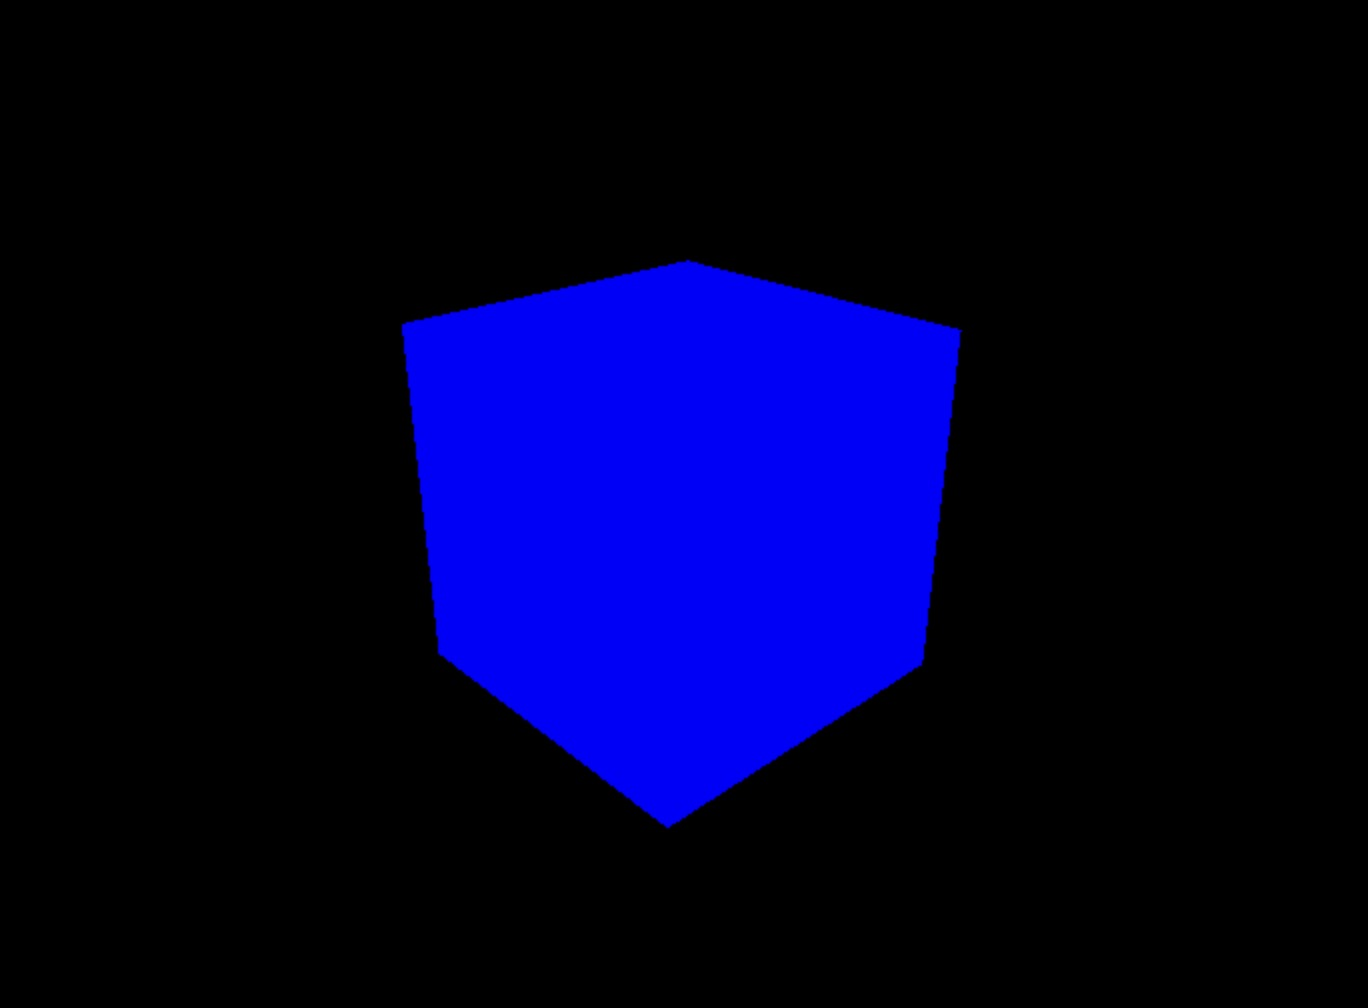
\includegraphics[width=1\linewidth]{graphics/boxGeometry}
\caption[BoxGeometry mesh visualisatie]{BoxGeometry mesh visualisatie}
\label{fig:boxGeometry}
\end{figure}

\newpage
\subsubsection{De camera}

Nu de mesh is toegevoegd aan de scene is de volgende stap een camera plaatsen in de scene. De camera is niet zichtbaar en is eerder een theoretisch 'punt' waaruit de render zal plaatsvinden. Er is ook een mogelijkheid om meerdere camera's te gebruiken maar dit is zeldzaam. Net zoals er vele soorten geometrieën en materialen zijn komen ook meerderde soorten camera's voor.

Bij het aanmaken van een camera zijn opnieuw twee vereisten: de 'field of view' of gezichtsveld en de 'aspect ratio' of beeldverhouding. 

Het gezichtsveld is de grootte van de hoek waarmee gekeken wordt, is de hoek groot dan zal alles vervormd worden op een manier dat het uitgezoomd lijkt. Als de hoek echter klein is dan lijkt het alsof er ingezoomd word. Een standaard waarde voor het gezichtsveld of 'FOV' is 75 graden en correspondeert met de verticale hoek.

De beeldverhouding wordt in de meeste gevallen bepaald door de breedte te delen door de hoogte. In volgend voorbeeld wordt getoond hoe een simpele PerspectiveCamera in de scene geplaatst wordt \autocite{Simon2023}.

\begin{LVerbatim}
const maten = {
	breedte: 800,
	hoogte: 600
}

const camera = new THREE.PerspectiveCamera(75, maten.breedte / maten.hoogte)
scene.add(camera)
\end{LVerbatim}

\subsubsection{De renderer}

Als laatste moet de scene weergegeven worden en dit kan a.d.h.v. een renderer. Dat doet de renderer door te communiceren met WebGL. Om de render te zien wordt een canvas element meegegeven aan de renderer als volgt: 

\begin{LVerbatim}
const canvas = document.querySelector('canvas.webgl')

const renderer = new THREE.WebGLRenderer({
	canvas: canvas
}
renderer.setSize(maten.breedte, maten.hoogte)

renderer.render(scene, camera)
\end{LVerbatim}

Nog een nodige stap om deze basis scene te zien is om de camera of de kubus van positie te veranderen omdat ze zich nu allebei in het midden bevinden. Dit kan simpelweg gedaan worden door de positie property van de camera te veranderen. Belangrijk is dat dit moet gedaan worden vooraleer de render uitgevoerd word \autocite{Simon2023}.

\begin{LVerbatim}

camera.position.z = 5

\end{LVerbatim}

\subsubsection{Transformaties}

Met transformaties kunnen bewerkingen uitgevoerd worden op de meshes die zich bevinden in de scene. Hiervoor zijn er 4 opties: 

\begin{itemize}
	\item positie
	\item schaal
	\item rotatie
	\item kwaternion
\end{itemize}

Deze opties spreken voor zichzelf, de positie bepaald waar de mesh zich bevind in de scene a.d.h.v. de x, y en z eigenschappen. Hiervoor gebruikt Three.js een Vector3 klasse, de positie is dus een instantie van de Vector3 klasse, zo is er ook de Vector2 klasse maar deze is minder voorkomend.

De schaal is ook een instantie van de Vector3 klasse en heeft dus ook x, y en z eigenschappen.

De rotatie van een mesh is een instantie van Euler i.p.v. Vector3 maar heeft ook x, y en z eigenschappen. Euler is een veel gebruikte manier van rotaties noteren in drie-dimensionale omgevingen, als men bijvoorbeeld de mesh 180 graden wil draaien op de x-as kan dat door Math.PI mee te geven aan de x-eigenschap van de rotatie.

Een kwaternion kan ook gebruikt worden om de rotatie van de mesh te bepalen maar is een stuk complexer, het voordeel van de kwaternion is dat het de vaste x, y en z assen vermijd \autocite{Simon2023}.

\subsubsection{Animaties}

Animaties zijn de strekte van Three.js, kort uitgelegd zijn animaties een transformatie uit voeren op een of meerder modellen en dan opnieuw een render uitvoeren. Stel dat een kubus zich bevindt op plaats (0, 0, 0) op de initiële render, wanneer de kubus een nieuwe positie krijgt bijvoorbeeld (5, 0, 0) zal de volgende render de kubus zich daar bevinden. 

Om de animaties er beter te laten uitzien heeft Three.js een oplossing ter beschikking. De klok maakt het gemakkelijk voor developers om goede animaties te maken omdat deze rekening houdt met de tijd die verstreken is. De native Javascript methode gebruikt de framerate van de gebruiker maar omdat dit kan verschillen zal geopteerd worden voor de klok.

De klok kan als volgt gebruikt worden:

\begin{LVerbatim}
const klok = new THREE.Clock()

const tick = () =>
{
	const elapsedTime = klok.getElapsedTime()
	
	// Update mesh
	mesh.position.x = Math.cos(elapsedTime)
}

tick()
\end{LVerbatim}

Met de getElapsedTime() methode kan de tijd die verstreken is gevraagd worden en zal de kubus op basis van deze tijd veranderen van positie. 

\subsubsection{Soorten camera's}

Three.js biedt een hoop camera's aan, in dit stuk worden de voornaamste vermeld.

De meeste gebruikte camera is de perspectief camera \ref{fig:perspectiefCamera}, die al eerder vermeld is, hiervoor is een gezichtsveld waarde nodig en een beeldverhouding waarde. De naam van de camera is vanzelfsprekend, wanneer deze gebruikt wordt dan zal de scene vanuit een perspectief bekeken worden. Dat wil zeggen dat het bekeken wordt vanaf 1 punt en waar dat punt is zal bepalen hoe de scene gerendered word.

De orthografische camera \ref{fig:orthografischeCamera} is nog een mogelijkheid, deze camera zal objecten renderen zodat de afstand van het object tot de camera geen invloed heeft op de grootte. Dit kan handig zijn voor 2D scenes of UI elementen te renderen \autocite{threejs2023}.

\begin{figure}
	\centering
	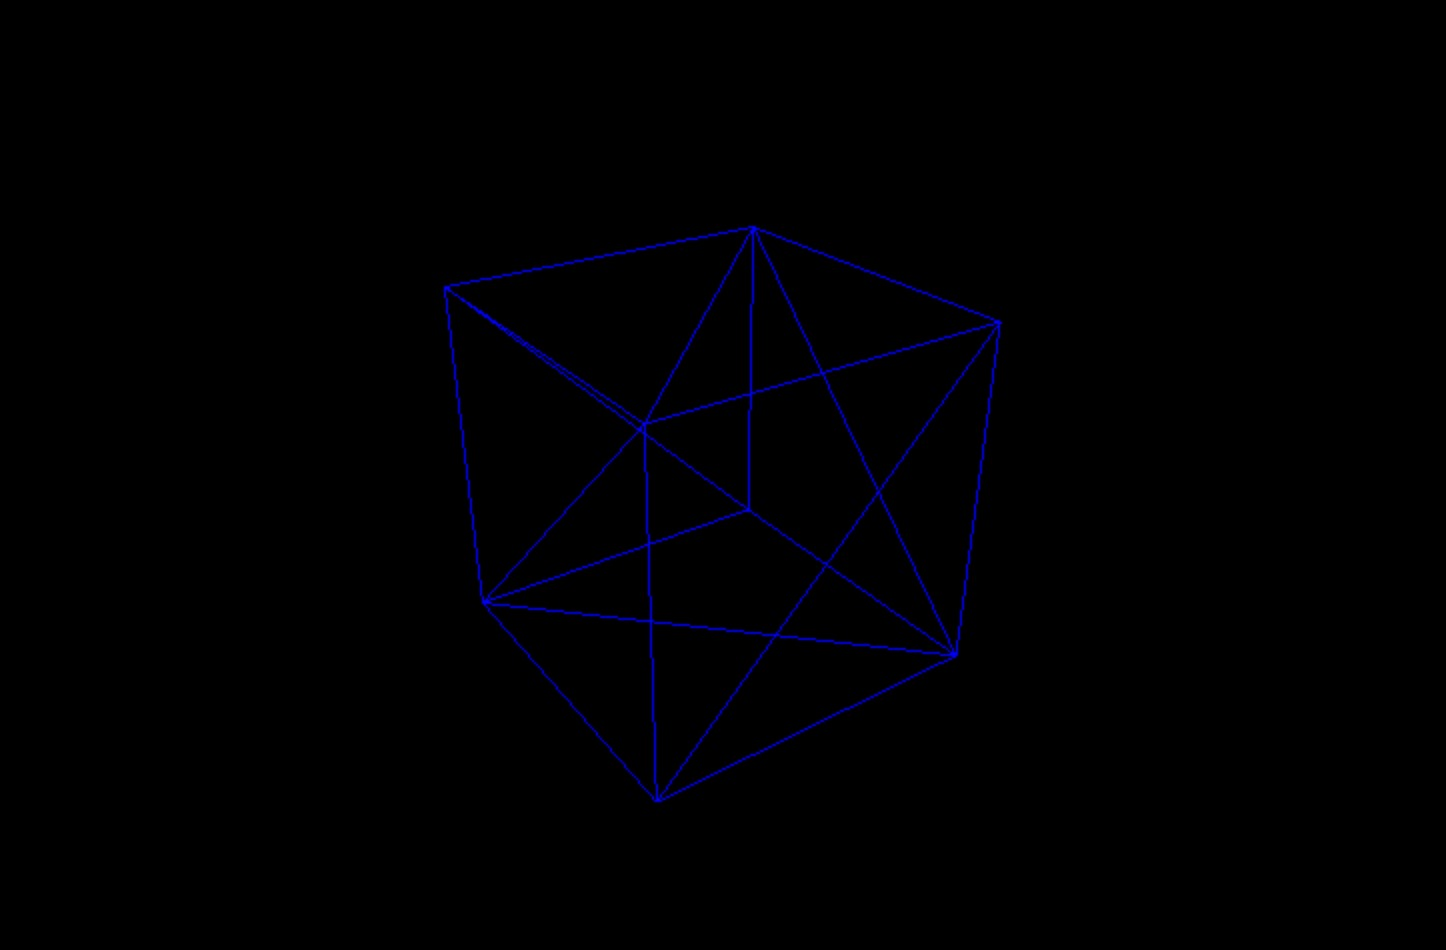
\includegraphics[width=1\linewidth]{graphics/perspectiefCamera}
	\caption[Perspectief camera visualisatie]{Perspectief camera visualisatie wireframe BoxGeometry}
	\label{fig:perspectiefCamera}
\end{figure}

\begin{figure}
	\centering
	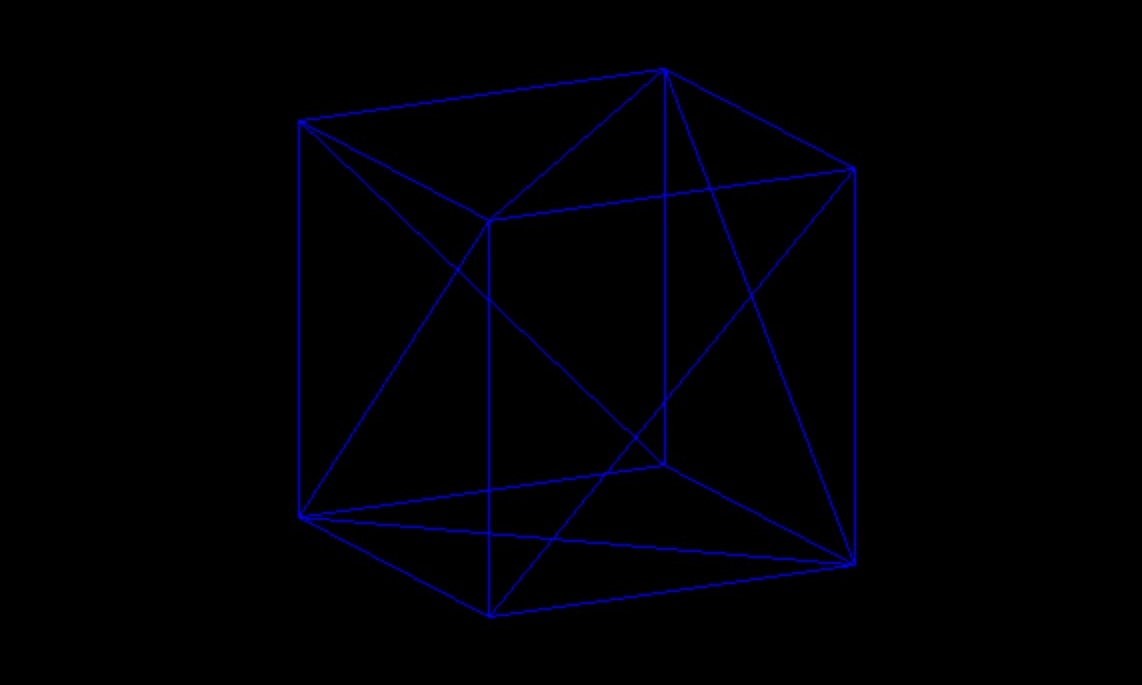
\includegraphics[width=1\linewidth]{graphics/orthografischeCamera}
	\caption[Orthografische camera visualisatie]{Orthografische camera visualisatie wireframe BoxGeometry}
	\label{fig:orthografischeCamera}
\end{figure}
\newpage
\subsubsection{Soorten geometriën}

De bibliotheek van Three.js heeft een veel basis geometriën waar developers gemakkelijk van gebruik kunnen maken. Tijdens het schrijven van deze scriptie zijn er 18 beschikbaar waaronder de BoxGeometry \ref{fig:boxGeometry}, PlaneGeometry, SphereGeometry, TextGeometry en nog meer.

Een geometrie in Three.js bestaat uit vertices en vlakken. Elke geometrie heeft in essentie een hoop driehoeken met 3 vertices of hoekpunten en een vlak. Wanneer deze driehoeken gecombineerd worden geeft het als resultaat een geometrie. Hiermee kan Three.js zeer complexe maar ook zeer simpele vormen representeren. Als voorbeeld kan een vlak genomen worden of in Three.js genaamd een PlaneGeometry \ref{fig:planeGeometry}, een vlak bestaat uit twee driehoeken en heeft dus 6 vertices. Een stap hoger is dan de BoxGeometry \ref{fig:boxGeometry} die 6 vlakken omvat en dus uit 12 driehoeken of 36 vertices bestaat. Nog een paar stappen hoger en dan kan een SphereGeometry \ref{fig:sphereGeometry} gemaakt worden, deze vorm is een stuk complexer want het lijkt alsof het een bol is maar in realiteit bestaat de bol uit een hoop vlakken en heeft dus veel meer driehoeken nodig om gerealiseerd te worden \autocite{threejs2023}.

Hoe meer driehoeken er gebruikt worden hoe meer detail de developer dus kan implementeren maar dit brengt een prijs met zich mee. Elke vertex heeft een coördinaat en moet gerendered worden, wanneer er animaties gebeuren in de scene en de developer is iets te enthousiast geweest dan kan al zeer snel een vertaging zijn. Zeker als we weten dat er nog veel computers zijn waar de GPU nog niet optimaal is, bijvoorbeeld op gsm's. Wanneer men dus met animaties werkt is het vaak een vuistregel om zo weinig mogelijk driehoeken te gebruiken voor de geometriën. Zo kan de beste omgeving voorzien worden om elke gebruiker de optimale ervaring te geven.

\begin{figure}
	\centering
	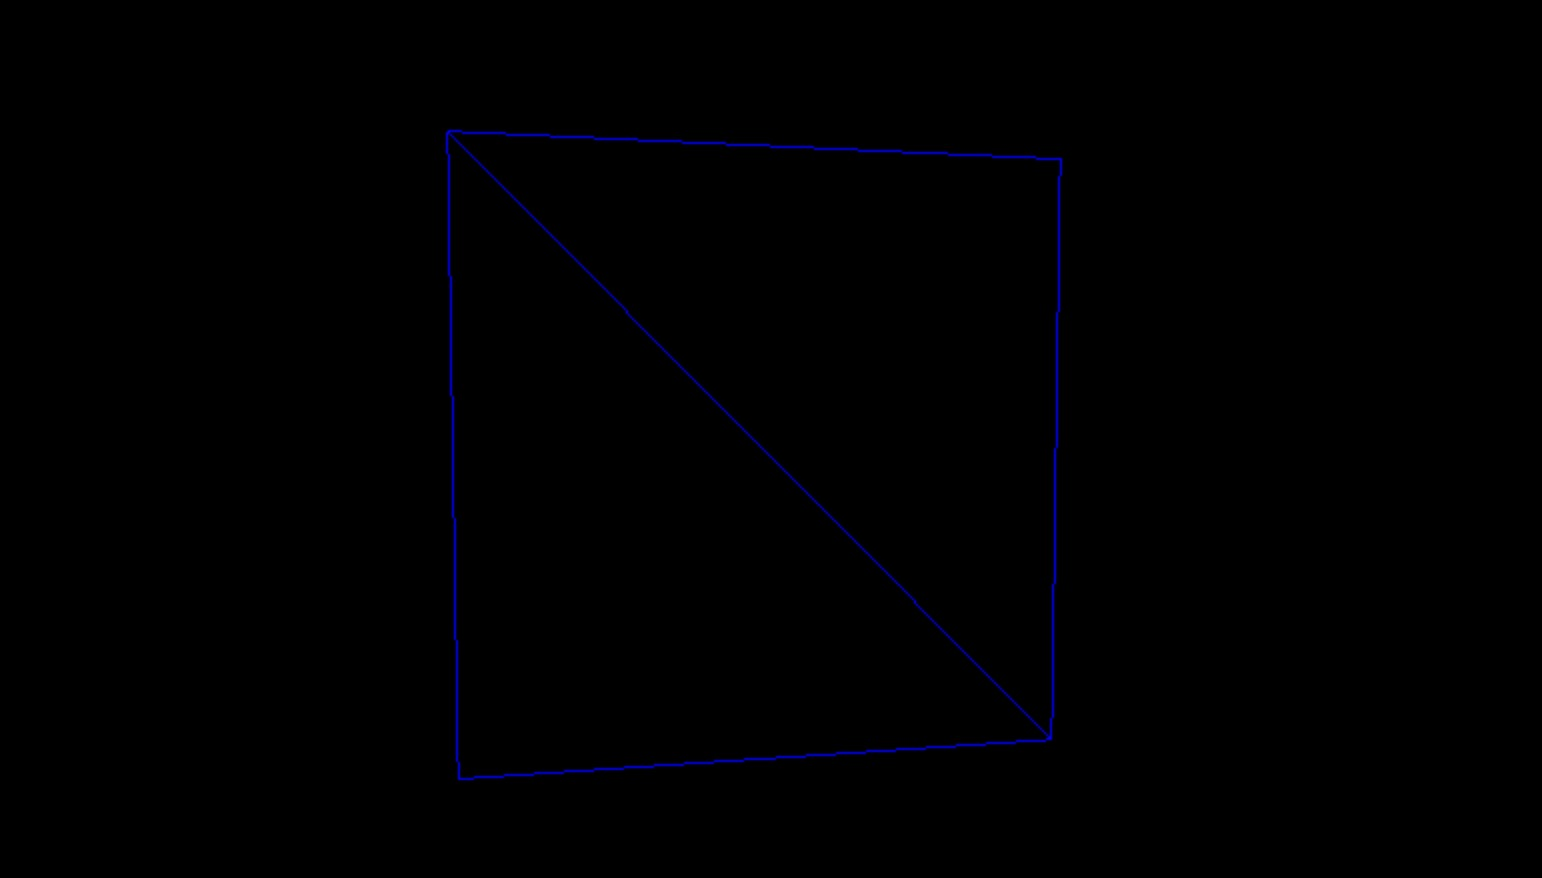
\includegraphics[width=1\linewidth]{graphics/planeGeometry}
	\caption[Visualisatie wireframe PlaneGeometry]{Visualisatie wireframe PlaneGeometry}
	\label{fig:planeGeometry}
\end{figure}

\begin{figure}
	\centering
	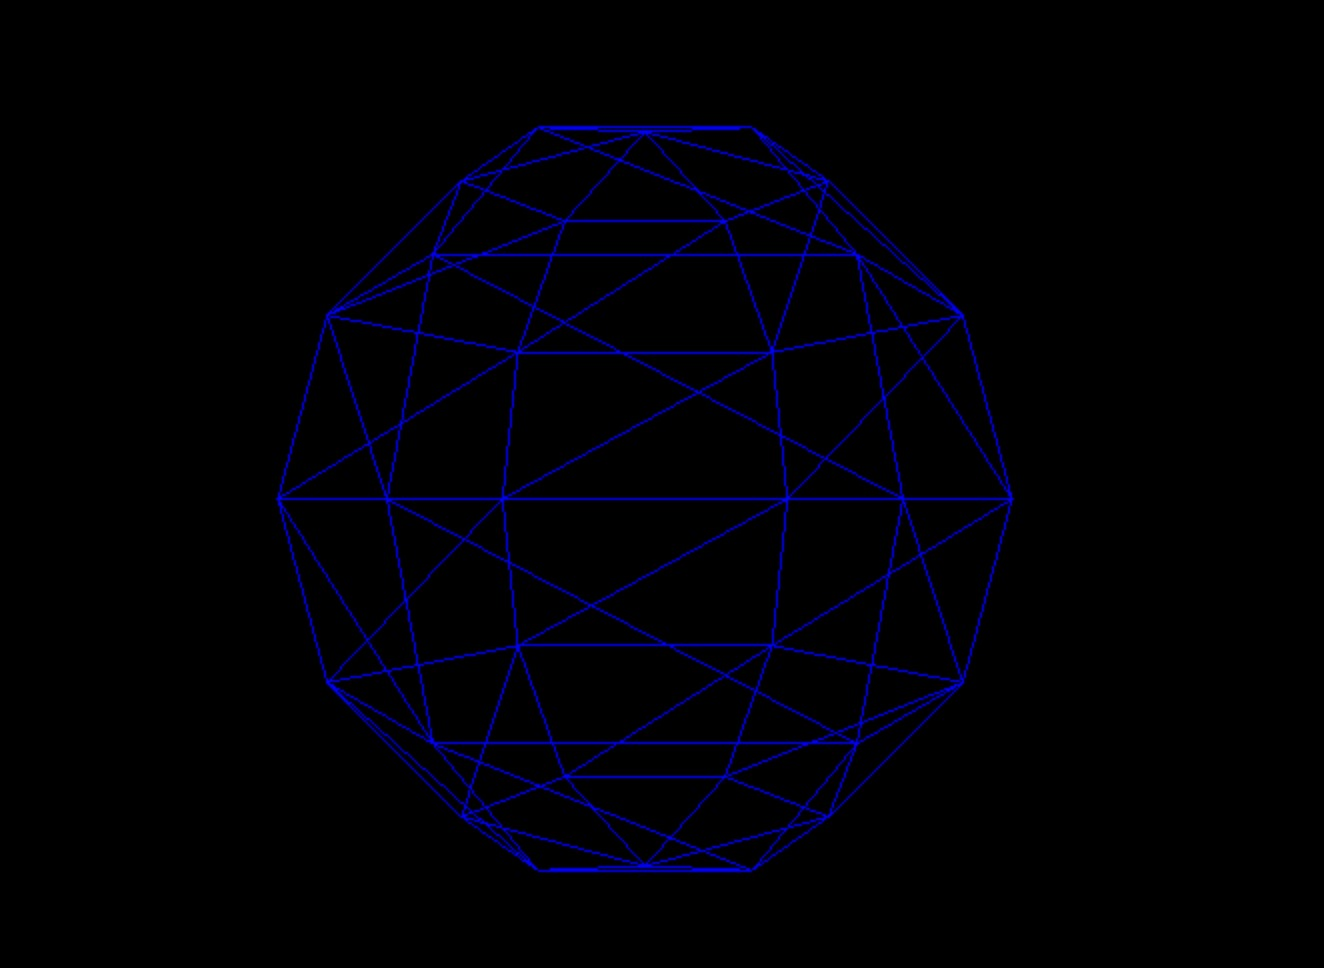
\includegraphics[width=1\linewidth]{graphics/sphereGeometry}
	\caption[Visualisatie wireframe SphereGeometry]{Visualisatie wireframe SphereGeometry}
	\label{fig:sphereGeometry}
\end{figure}

\newpage
\subsubsection{Texturen}

Texturen zijn afbeeldingen die over de vlakken van een geometrie gelegd worden. Hierbij bestaan de volgende soorten texturen: 

\begin{itemize}
\item Kleur of albedo
\item Alfa
\item Hoogte
\item Normaal
\item Omgevingsocclusie
\item Metaalheid
\item Ruwheid
\end{itemize}

Deze texturen bieden de mogelijkheid aan om een geometrie een realistisch uitzicht te geven. Met de kleur textuur zal elke pixel van de afbeelding geplakt worden op de geometrie. De alfa textuur is een grijstint afbeelding waar wit het zichtbare voorstelt en zwart hetgeen wat niet zichtbaar is voorstelt. De hoogte textuur is ook een grijstint afbeelding die a.d.h.v. de tinten een reliëf creëert in de geometrie. Hierbij zullen de vertices van plaats veranderd worden om dit effect te verwezenlijken. De normaal textuur voegt kleine details toe aan de geometrie en doet dit door het licht zodanig te manipuleren dat het denkt dat bepaalde vlakken of driehoeken anders georiënteerd zijn. De omgevingsocclusie textuur is opnieuw een grijstint afbeelding die valse schaduwen zal plakken in de gleuven van de geometrie, alhoewel dit niet echt is zorgt het voor een beter contrast. Met de metaaheid textuur, dat ook een grijstint afbeelding is, zullen de stukken van de geometrie die metaal zijn in het wit voorgesteld worden. Met deze info maakt Three.js deze delen van de geometrie meer reflectief. En dan is er tenslotte de ruwheid textuur die grijstinten gebruikt om op dezelfde manier als de metaalheid textuur delen van de geometrie een ruwheid te geven \autocite{Simon2023}.

Omdat texturen eigenlijk afbeeldingen zijn worden ze met normale Javascript code ingeladen. Ze worden in Three.js als volgt gedefinieerd:

\begin{LVerbatim}
const textuur = new THREE.Texture(afbeelding)
\end{LVerbatim}

\begin{figure}
	\centering
	\includegraphics[width=1\linewidth]{graphics/}
	\caption[]{}
	\label{fig:1}
\end{figure}
\begin{figure}
	\centering
	\includegraphics[width=1\linewidth]{graphics/}
	\caption[]{}
	\label{fig:2}
\end{figure}
\begin{figure}
	\centering
	\includegraphics[width=1\linewidth]{graphics/}
	\caption[]{}
	\label{fig:3}
\end{figure}
\begin{figure}
	\centering
	\includegraphics[width=1\linewidth]{graphics/}
	\caption[]{}
	\label{fig:4}
\end{figure}
\begin{figure}
	\centering
	\includegraphics[width=1\linewidth]{graphics/}
	\caption[]{}
	\label{fig:5}
\end{figure}
\begin{figure}
	\centering
	\includegraphics[width=1\linewidth]{graphics/}
	\caption[]{}
	\label{fig:6}
\end{figure}
\subsubsection{Materialen}

Materialen worden in Three.js gebruikt om een kleur te voorzien voor elke zichtbare pixel van een geometrie. De algoritmes die bepalen welke pixel welke kleur krijgt zijn geschreven in specifieke 'shader' programma's. Shaders schrijven is een uiterst complex gegeven en is dus zeker niet voor iedereen weggelegd maar gelukkig biedt Three.js materialen aan met ingebouwde shaders \autocite{Simon2023}.

Een materiaal zal de textuur mappen op de geometrie en daarvoor hoeft de developer niet veel te doen. Het kan op de volgende manier gedaan worden:

\begin{LVerbatim}
const materiaal = new THREE.MeshBasicMaterial({ map: textuur })
\end{LVerbatim}

Voor de verschillende soorten texturen zijn ook methodes voorzien om ze correct te plaatsen op de geometrie.

\subsubsection{Tekst geometrie}

De tekst geometrie genereert kort gezegd 3D tekst. Deze geometrie werkt bijna exact hetzelfde als de andere en wordt gebruikt om tekst te plaatsen in een scene. De extra stap die genomen moet worden is om een font mee te geven bij de initialisatie, daarvoor moet eerst een FontLoader aangemaakt worden om de font in te laden. Vervolgens kan dan de font ingeladen worden.

\begin{LVerbatim}
const fontLoader = new THREE.FontLoader()

// Inladen font
const fontKeuze = fontloader.load('/fonts/fontNaarKeuze.typeface.json')
\end{LVerbatim}

Nu de font ingeladen is kan de tekst geometrie geïnitialiseerd en uiteraard ook toegevoegd worden aan de scene. Dit wordt als volgt gedaan:

\begin{LVerbatim}
const textGeometrie = new THREE.TextGeometry('Hello World', { font: fontKeuze })
const textMateriaal = new THREE.MeshBasicMaterial()

const text = new THREE.Mesh(textGeometrie, textMateriaal)
scene.add(text)
\end{LVerbatim}

\subsection{Klassieke Technieken}

In dit hoofdstuk worden de technieken overlopen in Three.js die niet noodzakelijk zijn om een scene te maken maar wel zorgen voor een aanzienlijke meerwaarde.

\subsubsection{Lichten}

Met licht kan in een scene een compleet ander perspectief gegeven worden aan meshes. Hierbij zijn er een aantal lichten die ter beschikking gesteld zijn waaronder:

\begin{itemize}
	\item AmbientLight
	\item DirectionalLight
	\item HemisphereLight
	\item PointLight
	\item RectAreaLight
	\item SpotLight
\end{itemize}

Omdat AmbientLight of omgevingslicht en DirectionalLight of directioneel licht de voornaamste zijn die gebruikt worden binnen Three.js zullen deze uitgediept worden. Uitleg over de andere soorten licht is te vinden op de documentatie van Three.js.

Belangrijk is dat materialen verschillend kunnen reageren op licht, het MeshBasicMaterial bijvoorbeeld is niet beïnvloed door licht. Er moet dus een andere soort materiaal gebruikt worden, hiervoor kan MeshStandardMaterial op de mesh toegepast worden. Bij dit materiaal is het aangeraden om een licht te gebruiken want indien dat niet het geval is zal de mesh ook niet zichtbaar zijn \autocite{Simon2023}.

\subsubsection{AmbientLight}

AmbientLight of omgevingslicht geeft omnidirectioneel licht op alle meshes die zich in de scene bevinden. Het initialiseren van dit licht vergt twee parameters zijnde de kleur en intensiteit.

\begin{LVerbatim}
const omgevingslicht = new THREE.AmbientLight(0x00ff00, 0.5)
scene.add(omgevingslicht)
\end{LVerbatim}

\subsubsection{DirectionalLight}

DirectionalLight of directioneel licht kan je vergelijken met zonlicht, alle stralen komen parallel vanuit dezelfde richting maar geen specifiek punt. Hierbij kan je de positie aanpassen net zoals de positie van de zon ook kan veranderen, bij initialisatie wordt ook de kleur en intensiteit meegegeven.

\begin{LVerbatim}
const directioneelLicht = new THREE.DirectionalLight(0xff0000, 0.4)
scene.add(directioneelLicht)
\end{LVerbatim}

De positie kan op de volgende simpele manier na initialisatie veranderd worden.

\begin{LVerbatim}
directioneelLicht.position.set(1, .5, 0)
\end{LVerbatim}

Lichten kunnen ook gecombineerd worden om een realistisch beeld te verkrijgen  \autocite{Simon2023}.

\subsubsection{Helpers}

Omdat het soms moeilijk kan zijn om een goed beeld te krijgen over waar een licht staat in de scene is het handig om een helper te gebruiken. Deze zal als een hulplijn dienen om de gewenste positie en dus resultaat te verkrijgen.

\subsubsection{Schaduwen}

Met de inbreng van licht krijgen we uiteraard ook schaduwen, de achterkant van de objecten is donker maar dit noemt men de kernschaduw. Hetgeen wat nog mist is de slagschaduw, hierbij zorgen meshes voor schaduwen op andere meshes.

De keerzijde van het implementeren van schaduwen is dat ze moeilijk te verkrijgen zijn aan een frame rate die goed is. Developers zullen dus creatieve oplossingen moeten vinden om een degelijke frame rate te verkrijgen \autocite{Simon2023}.

Er zijn drie soorten lichten die het gebruik van schaduwen mogelijk maken, deze zijn DirectionalLight, PointLight en SpotLight. In deze scriptie zal alleen DirectionalLight behandeld worden.

De schaduwen moeten eerst als volgt aangezet worden:

\begin{LVerbatim}
renderer.shadowMap.enabled = true
\end{LVerbatim}

Vervolgens moet doorheen elk object in de scene gegaan worden en bepaald worden of de mesh een schaduw moet maken, krijgen of beide. Dit moet ook bepaald worden voor het licht.

\begin{LVerbatim}
mesh.castShadow = true
mesh.receiveShadow = true

directioneelLicht.castShadow = true
\end{LVerbatim}

Voor performantie is de standaard waarde voor de schaduw map 512x512, voor meer gedetailleerde schaduwen kan de schaduw map grootte verhoogd worden met een macht van twee.

\begin{LVerbatim}
directioneelLicht.shadow.mapSize.width = 1024
directioneelLicht.shadow.mapSize.height = 1024
\end{LVerbatim}

Over schaduwen kan nog veel meer gezegd worden. Zo kan men bijvoorbeeld i.p.v. de schaduw te genereren een versie 'bakken' in een afbeelding en de op de mesh plakken, maar dit is al een stuk geavanceerder \autocite{Simon2023}.

\subsubsection{Fysica}

Fysica implementeren in een scene kan veel interactie geven aan de gebruiker. Zwaartekracht krijgt hier de hoofdrol en zal botsingen tussen de meshes veroorzaken. Dit gebeurd echter niet in een normale scene maar in een aparte wereld waar de krachten gesimuleerd worden. Deze wereld is puur theoretisch en kan niet gezien worden. Wanneer er een mesh wordt aangemaakt zal dezelfde versie van de mesh geïnitialiseerd worden in de natuurkundige wereld.
Op elke frame voor de render is uitgevoerd zal deze wereld een update krijgen en worden de nieuwe coördinaten van de mesh gelijk gemaakt aan de mesh in de normale scene. Dit is de enige vereiste \autocite{Simon2023}.

\subsection{React Three Fiber}

React Three Fiber is een bibliotheek die Three.js en React combineert zonder limieten, alles dat werkt in Three.js kan dus ook werken a.d.h.v. R3F. De manier hoe het werkt is dat Three.js vertaald wordt naar JSX, <mesh /> zal automatisch veranderen in new THREE.Mesh() \autocite{reactThreeFiber2023}.

\subsubsection{Canvas}

Via het Canvas object geeft R3F toegang tot de Three.js bibliotheek door een scene en renderer aan te maken. Binnen in het Canvas object kunnen dan alle andere delen geplaatst worden om een volledige ervaring te maken. In volgend voorbeeld word een Canvas object gebruikt in een React omgeving \autocite{reactThreeFiber2023}.

\begin{LVerbatim}
<Canvas camera={{ position: [0, 0, 25] }} >
	<mesh/>
</Canvas>
\end{LVerbatim}

Bij dit object kan dus ook een camera positie meegegeven worden maar ook andere props die te vinden zijn in de documentatie van R3F

\subsubsection{Objecten}

Een logische reactie zou zijn om als volgt props mee te geven aan een object:

\begin{LVerbatim}
<mesh
	position={new THREE.Vector3(2, 5, 8)}
	geometry={new THREE.BoxGeometry(10, 10, 10)}
	material={new THREE.MeshStandardMaterial({ color: new THREE.Color('red')})}
/>
\end{LVerbatim}

Het probleem met deze manier van werken is dat all deze props opnieuw aangemaakt zullen worden door R3F. De correcte manier in R3F om props mee te geven aan een object is dus als volgt:

\begin{LVerbatim}
<mesh position={[2, 5, 8]}>
	<boxGeometry args={[10, 10, 10]} />
	<meshStandardMaterial color="red" />
</mesh>
\end{LVerbatim}

Merk ook op dat de constructor argumenten voor het aanmaken van de BoxGeometry meegegeven worden in een 'args' prop. Voor alle argument van een object waar een set() methode kan op uitgevoerd worden kan dit wel als prop meegegeven worden bij de initializatie zoals de positie of kleur \autocite{reactThreeFiber2023}.

\subsubsection{Hooks}

De belangrijkste hook voor R3F is useThree(), deze hook geeft een developer toegang tot de state die de renderer, scene en camera bevat alsook de grootte van het canvas in scherm en viewport coördinaten. Deze hook kan echter niet aangeropen worden buiten de context van het Canvas object.

De volgende hook in de lijst is useFrame() waar de state en een klok delta uit gehaald kan worden. Binnenin de hook kan op elke frame een stuk code uitgevoerd worden net voor de frame is gerendered. Hier moet dus extra aandacht gehecht worden aan welk soort code geschreven wordt om eventuele loops te vermijden want dit kan een zeer zware impact hebben op de GPU.

De useLoader() hook gebruikt R3F voor het inladen van bepaalde textures, fonts of modellen a.d.h.v. een TextureLoader, FontLoader, GLTFLoader of OBJLoader.

%%=============================================================================
%% Methodologie
%%=============================================================================

\chapter{\IfLanguageName{dutch}{Methodologie}{Methodology}}%
\label{ch:methodologie}

%% TODO: Hoe ben je te werk gegaan? Verdeel je onderzoek in grote fasen, en
%% licht in elke fase toe welke stappen je gevolgd hebt. Verantwoord waarom je
%% op deze manier te werk gegaan bent. Je moet kunnen aantonen dat je de best
%% mogelijke manier toegepast hebt om een antwoord te vinden op de
%% onderzoeksvraag.
\section{Inleiding}

In dit onderdeel wordt de onderzoeksaanpak besproken. Dit zal een overzicht voorleggen van de  nodige stappen die ondernomen worden om de POC's en vergelijkende studie te realiseren.

Bij de start van het onderzoek wordt de eerste POC opgemaakt omdat hiervoor geen vereiste kennis nodig is over Three.js. Zo kan deze conventionele versie als een basis dienen voor de tweede POC. Beide POC's dienen zo identiek mogelijk te zijn waarbij het verschil ligt bij de implementatie van Three.js.

Het concept voor beide webshops is een online vinyl winkel, hierbij zal gebruik gemaakt worden van de Spotify API. Deze API zal voornamelijk benut worden om mockdata te voorzien. De keuze voor een vinyl webwinkel is omdat de 3D modellen die gebruikt zullen worden relatief simpel zijn.

\section{Mock-ups}

Alvorens er een lijn code geschreven wordt zijn er mock-ups gemaakt voor de mobiele versie \ref{fig:mobileMockUps} en de desktop versie, beide voor de Home Pagina \ref{fig:desktopHomeMockUp} en de Detail Pagina \ref{fig:desktopDetailMockUp}. Zoals eerder vermeldt dienen de mock-ups als een basis voor de conventionele versie van de webshop om een goede UX/UI te voorzien.

\begin{figure}
	\centering
	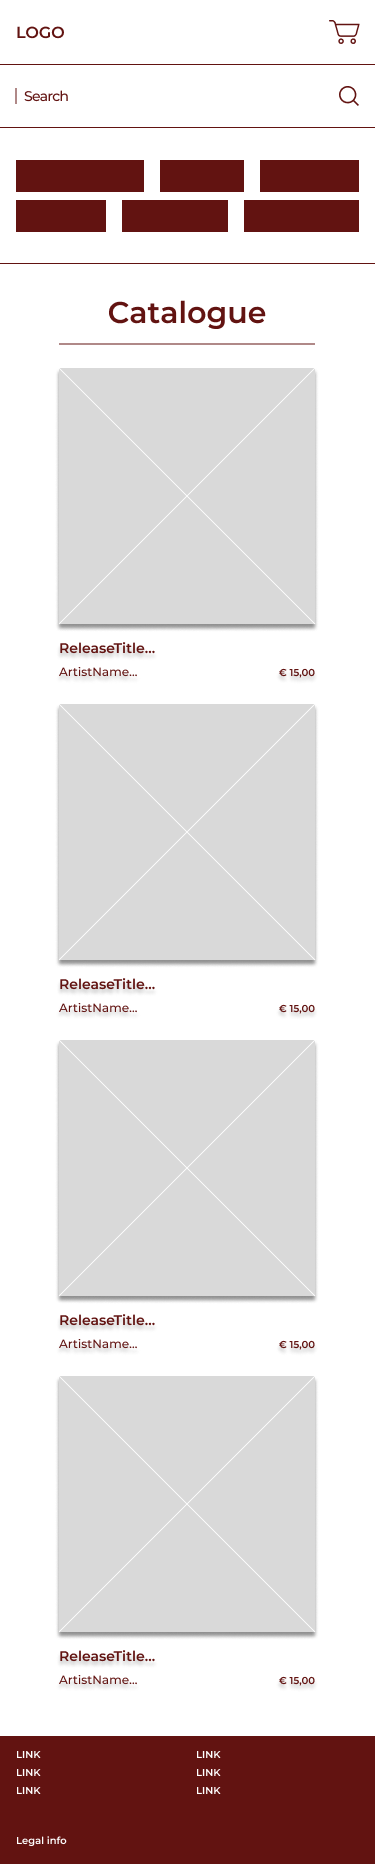
\includegraphics[width=0.3\linewidth]{graphics/HomePageMobile}
	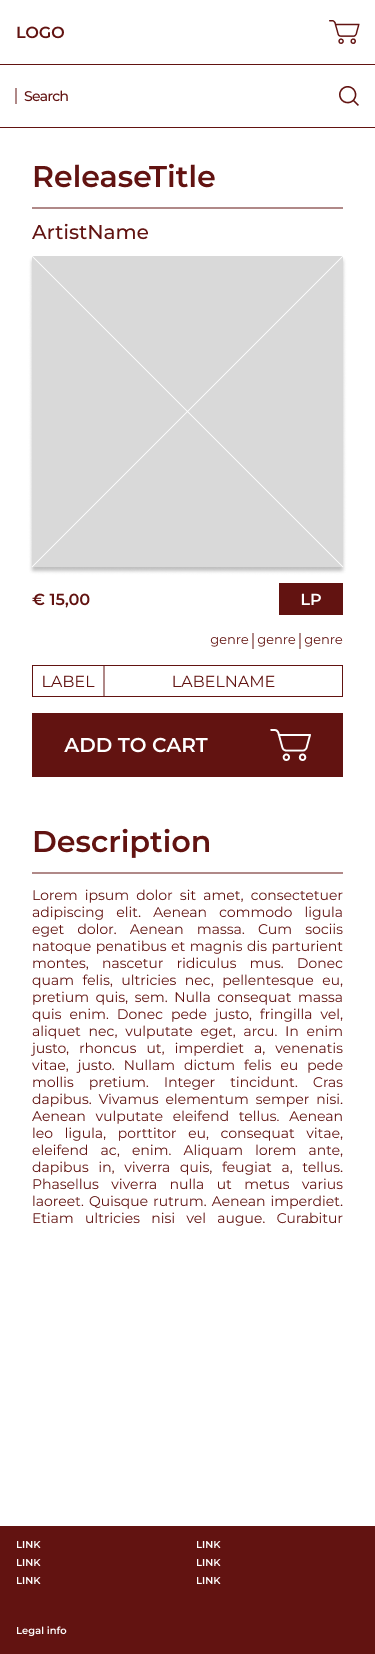
\includegraphics[width=0.3\linewidth]{graphics/DetailsPageMobile}
	\caption[Mock-Ups Mobile]{Mock-Ups Mobile}
	\label{fig:mobileMockUps}
\end{figure}

\begin{figure}
	\centering
	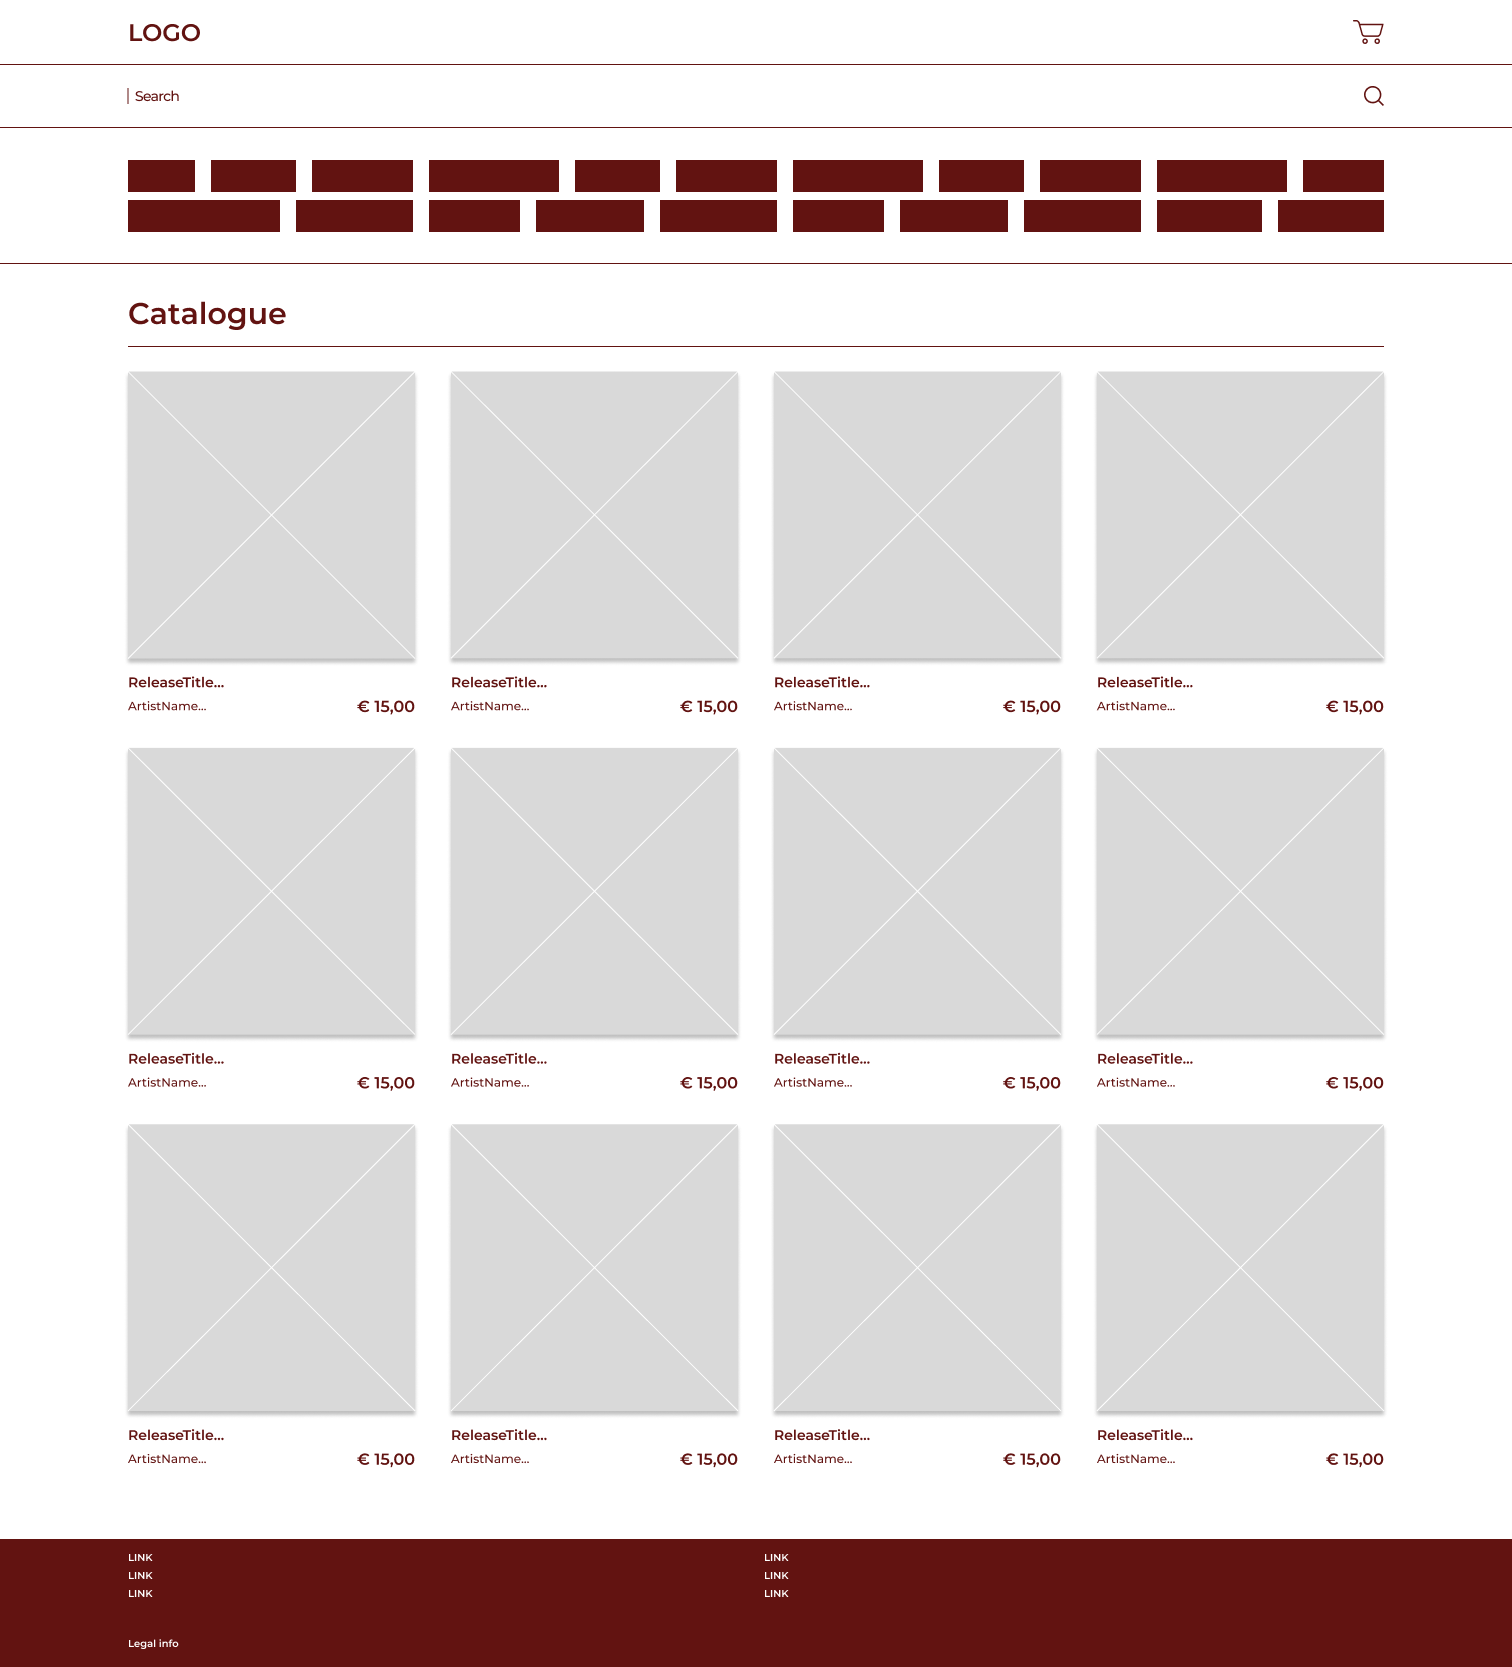
\includegraphics[width=1\linewidth]{graphics/HomePageDesktop}
	\caption[Mock-Up Desktop]{Mock-Up Desktop Home Pagina}
	\label{fig:desktopHomeMockUp}
\end{figure}

\begin{figure}
	\centering
	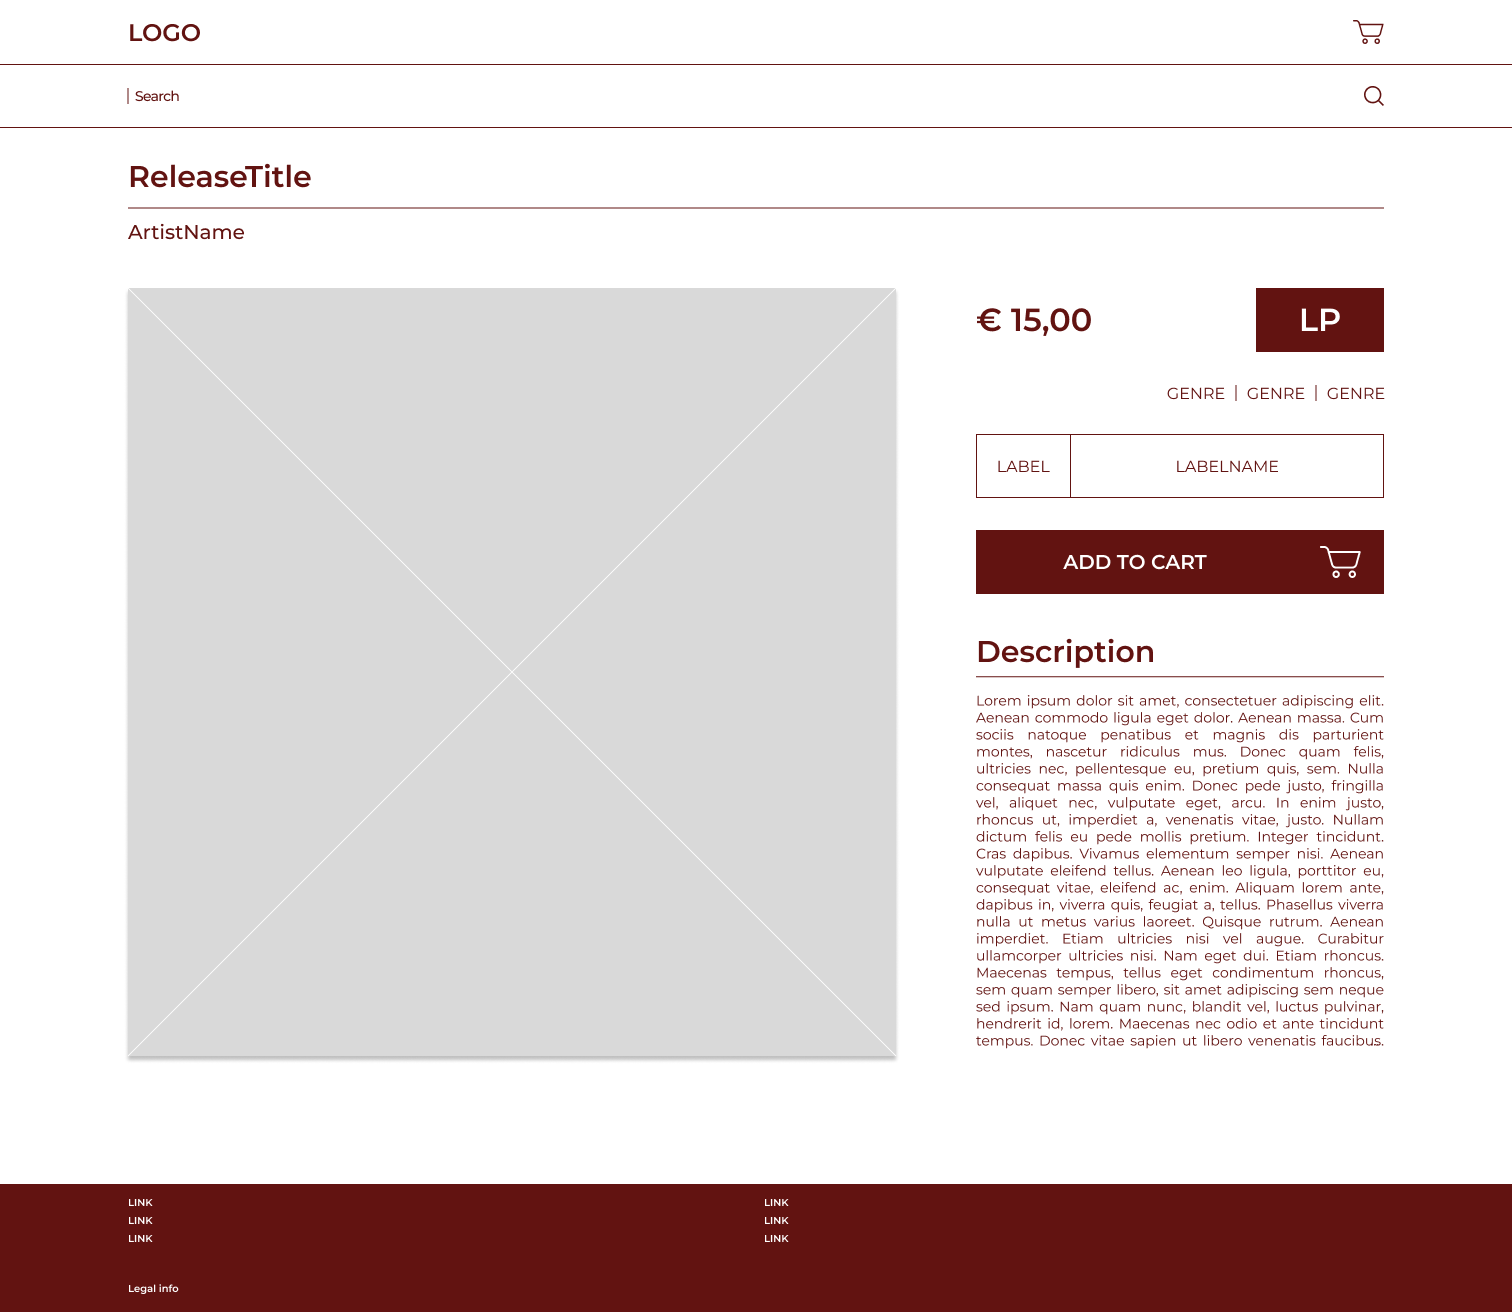
\includegraphics[width=1\linewidth]{graphics/DetailPageDesktop}
	\caption[Mock-Up Desktop]{Mock-Up Desktop Detail Pagina}
	\label{fig:desktopDetailMockUp}
\end{figure}

\pagebreak

\section{Proof-of-concept: Conventioneel}

De conventionele POC is de eerste die zal verwezenlijkt worden. Deze zal bestaan uit een React front-end en een Node.js backend om de Spotify API te hanteren. De reden voor het gebruiken van React en Node.js is omdat ze behoren tot de meest gebruikte frameworks voor het bouwen van websites.

Voor een goede flow te voorzien zijn een aantal user stories opgemaakt voor het concept van de vinyl webshop. Deze zijn:

\begin{itemize}
	\item Als Klant wil ik gemakkelijk navigeren door de selectie van vinyl op de webshop, filterende op artiest, album titel, etc., zodat ik de releases die ik wil snel kan terugvinden.
	\item Als Klant wil ik gedetailleerde informatie kunnen zien over elke release zodat ik een geïnformeerde beslissing kan maken of ik de release al dan niet zal kopen.
\end{itemize}

Om een degelijke webshop te realiseren worden de mock-ups als basis gebruikt. De reden hiervoor is omdat een goede UX/UI nodig is voor beide POC's. De inhoud en opbouw van deze POC wordt uitgebreid uitgelegd in volgend hoofdstuk~\ref{ch:proofofconceptConventioneel}

\section{Proof-of-concept: Three.js}

De POC die gebruik maakt van Three.js zal dus beginnen vanaf een kopie van de conventionele POC. Hierbij zullen een aantal aanpassingen gemaakt worden aan de webshop die van de technologie gebruik maken. Er wordt geprobeerd om zo dicht mogelijk te blijven bij de conventionele POC om een correcte vergelijkende studie uit te voeren.

De inhoud en opbouw van deze POC wordt uitgebreid uitgelegd in volgend hoofdstuk~\ref{ch:proofofconceptThreeJS}

% Voeg hier je eigen hoofdstukken toe die de ``corpus'' van je bachelorproef
% vormen. De structuur en titels hangen af van je eigen onderzoek. Je kan bv.
% elke fase in je onderzoek in een apart hoofdstuk bespreken.

%%=============================================================================
%% Proof-of-concept: Conventioneel
%%=============================================================================

\chapter{\IfLanguageName{dutch}{Proof-of-concept: Conventioneel}{Proof-of-concept: Conventional}}%
\label{ch:proofofconceptConventioneel}

\section{Inleiding}

In dit hoofdstuk zal een overzicht gegeven worden over hoe de conventionele webshop is opgebouwd. Hier zal echter niet dieper ingaan op het technische aspect van de React componenten of de API-calls die gerealiseerd zijn.

\section{Mock-ups}

Alvorens er een lijn code geschreven wordt zijn er mock-ups gemaakt voor de mobiele versie \ref{fig:mobileMockUps} en de desktop versie, beide voor de Home Pagina \ref{fig:desktopHomeMockUp} en de Detail Pagina \ref{fig:desktopDetailMockUp}. Zoals eerder vermeld dienen de mock-ups als een basis voor de conventionele versie van de webshop om een goede UX/UI te voorzien.

\begin{figure}
	\centering
	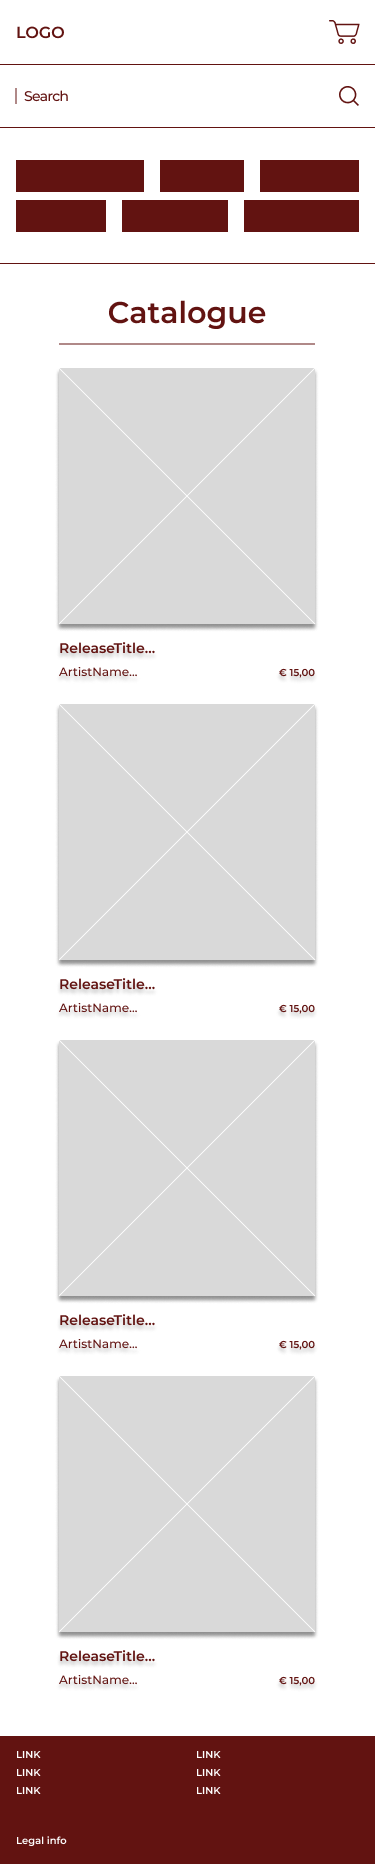
\includegraphics[width=0.3\linewidth]{graphics/HomePageMobile}
	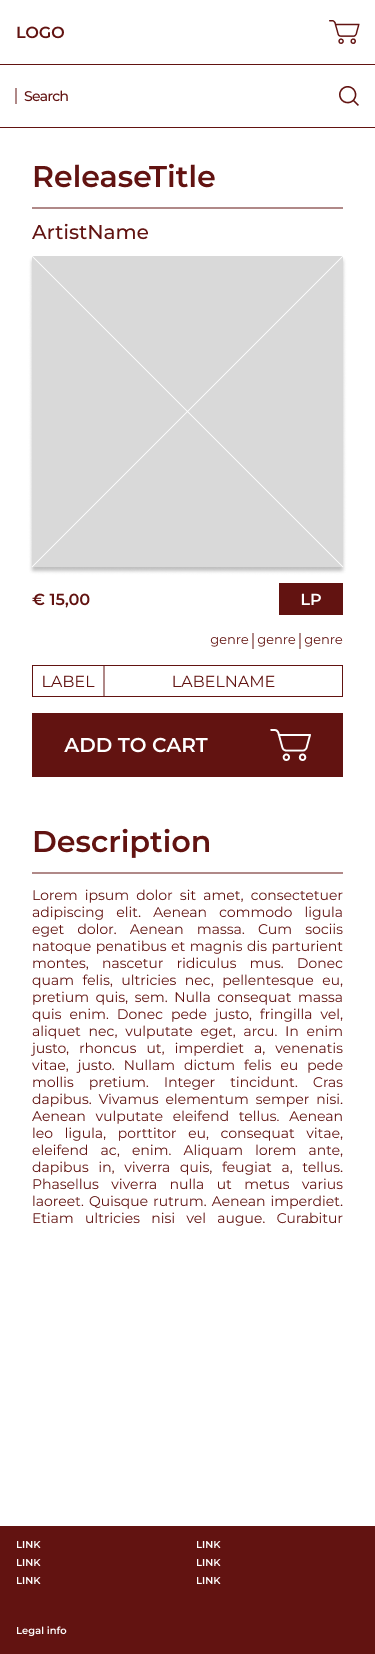
\includegraphics[width=0.3\linewidth]{graphics/DetailsPageMobile}
	\caption[Mock-Ups Mobile]{Mock-Ups Mobile}
	\label{fig:mobileMockUps}
\end{figure}

\begin{figure}
	\centering
	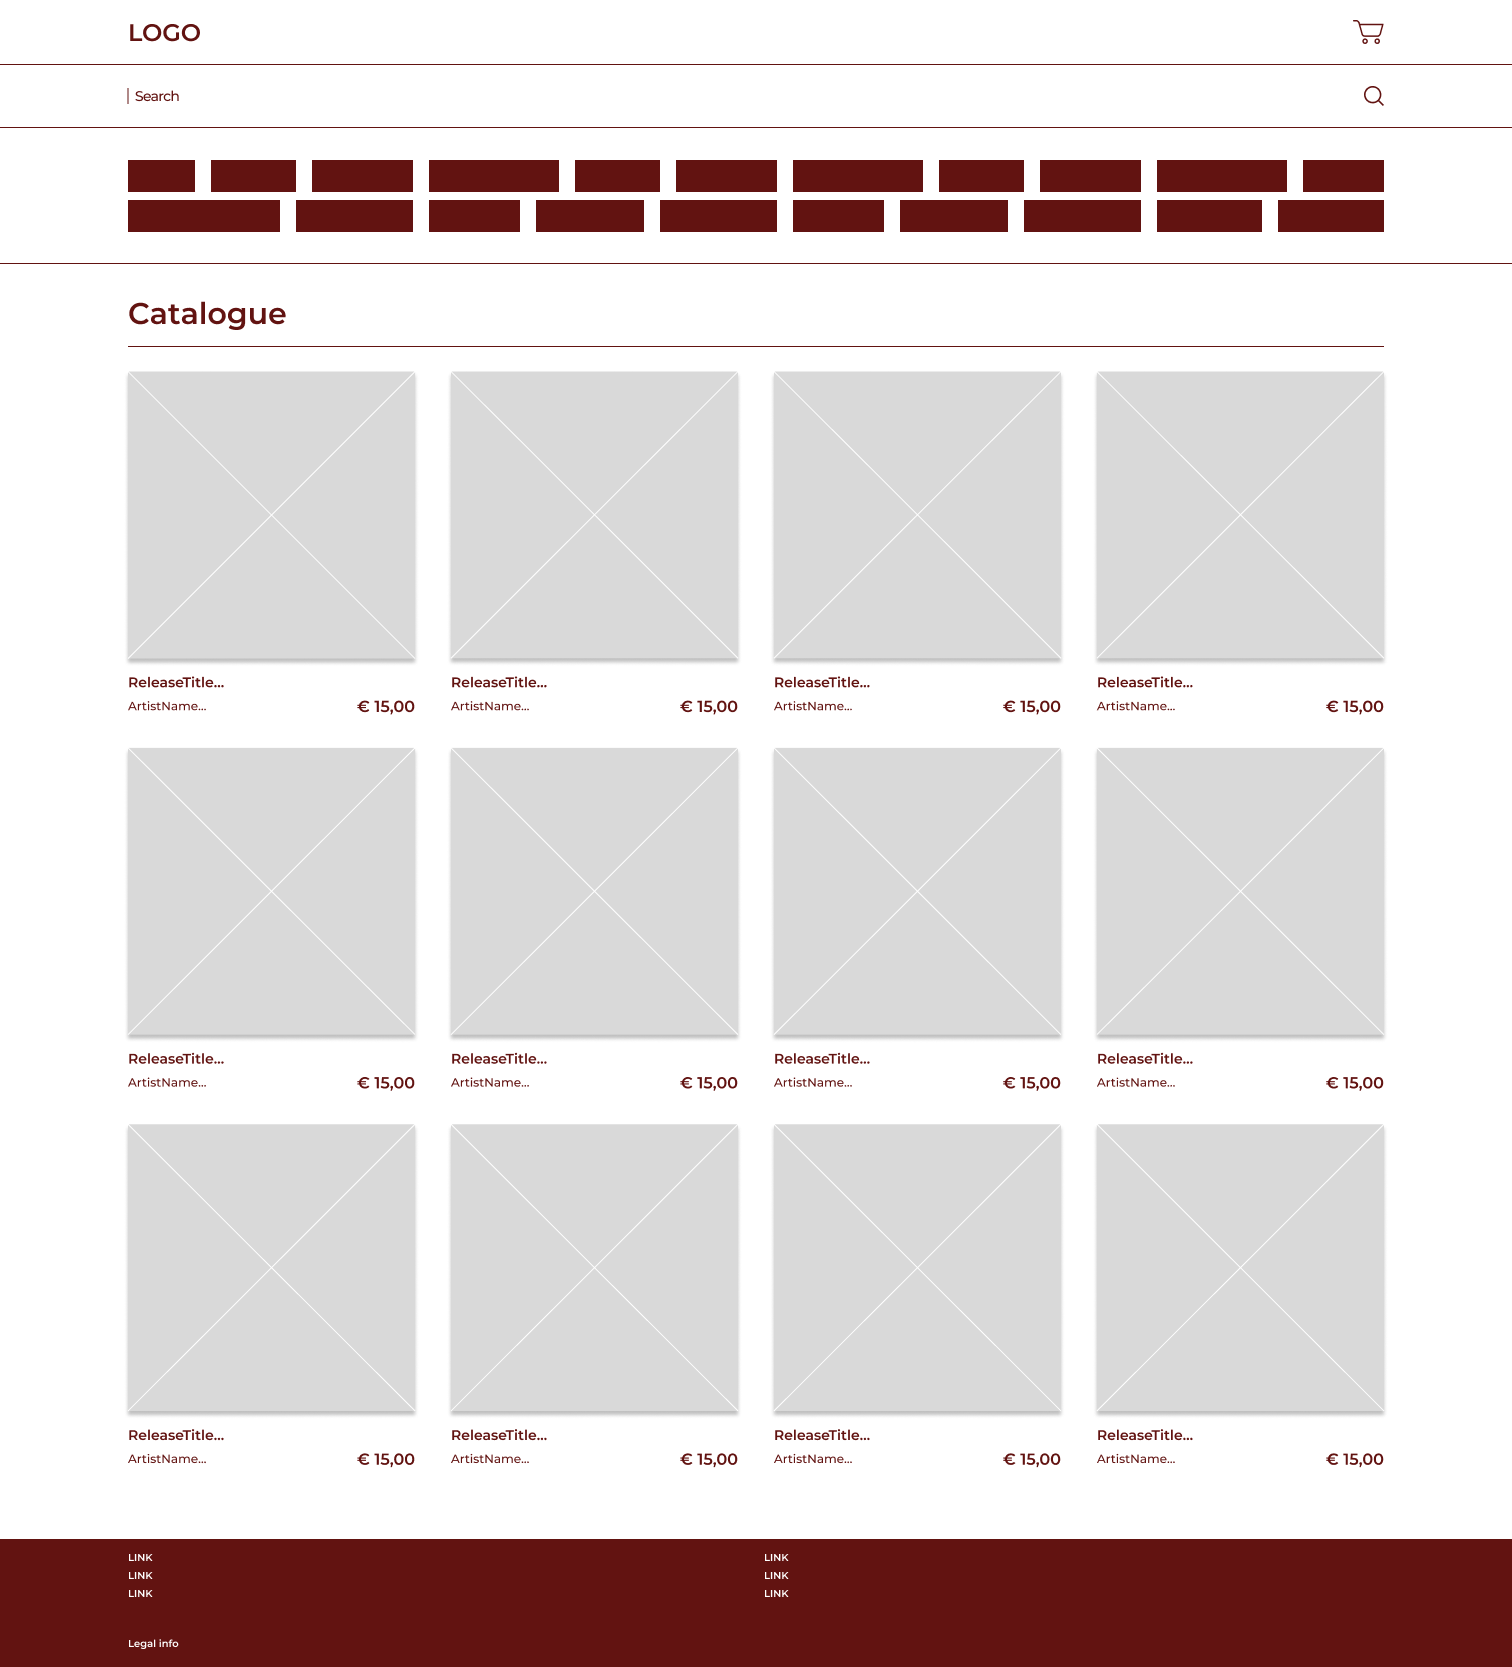
\includegraphics[width=1\linewidth]{graphics/HomePageDesktop}
	\caption[Mock-Up Desktop]{Mock-Up Desktop Home Pagina}
	\label{fig:desktopHomeMockUp}
\end{figure}

\begin{figure}
	\centering
	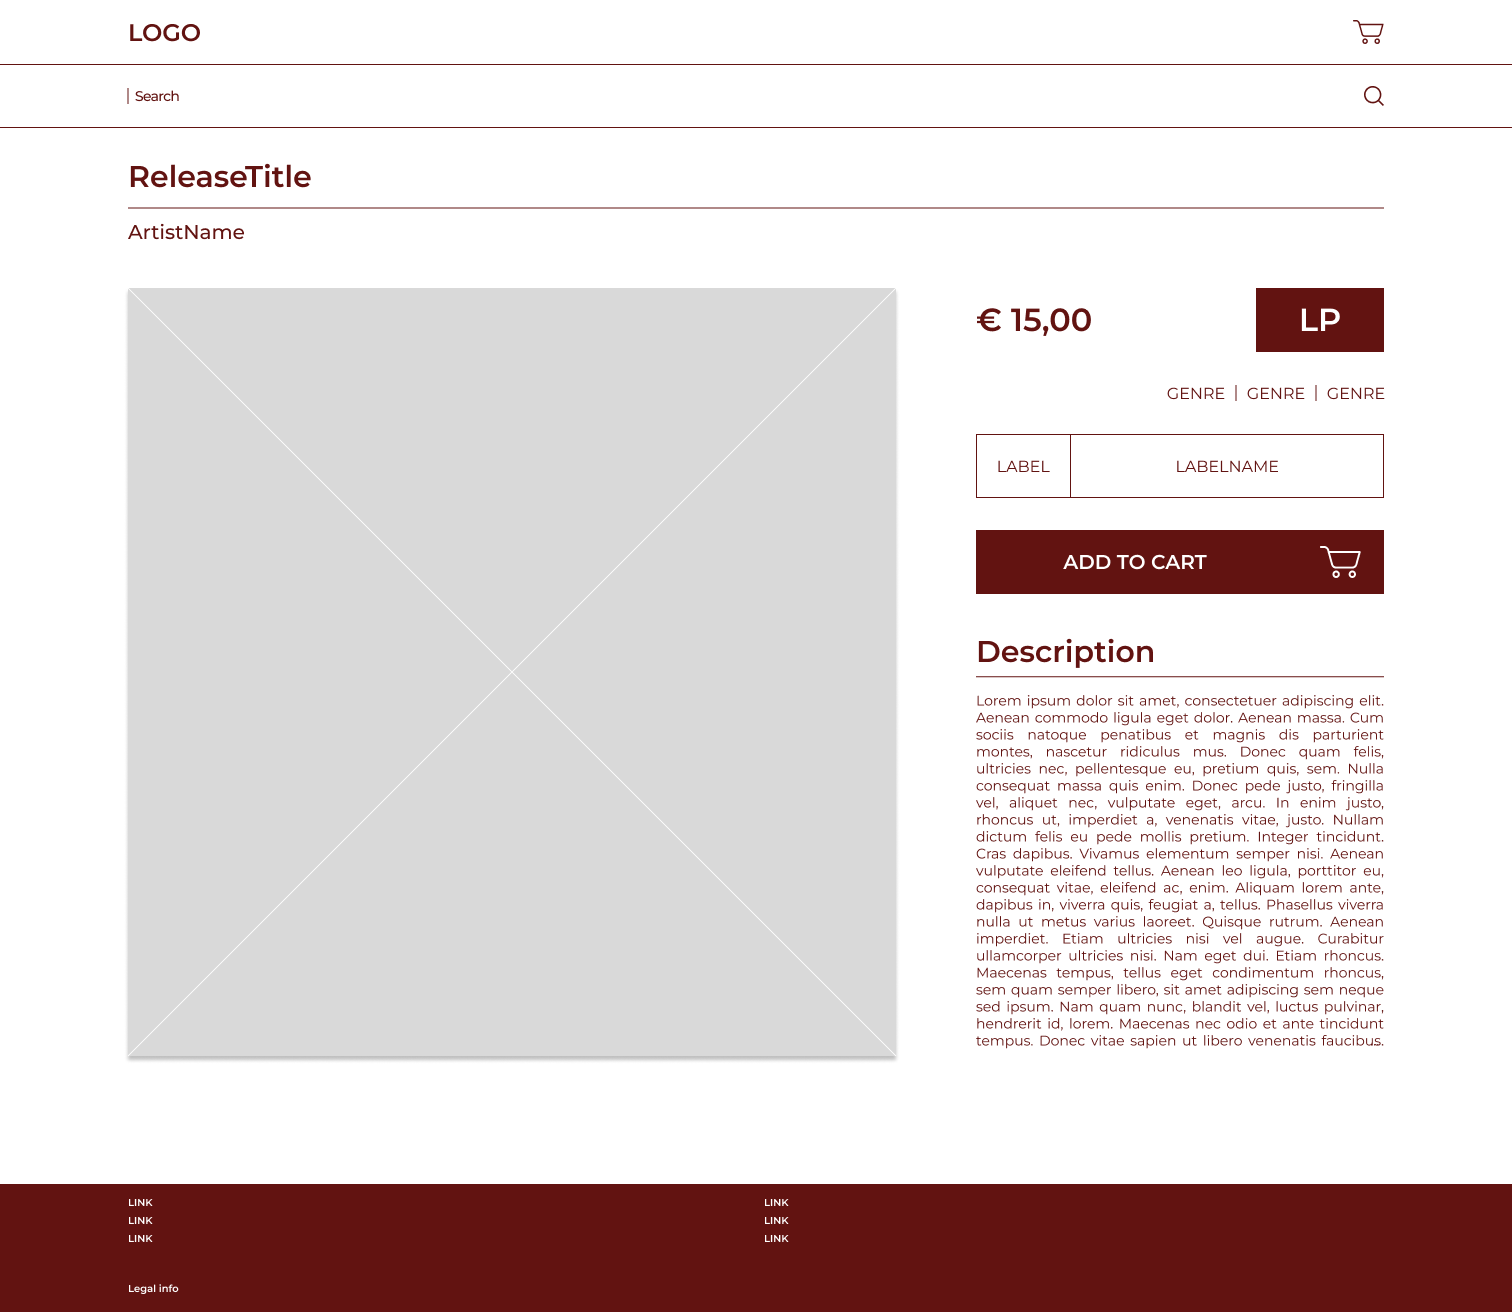
\includegraphics[width=1\linewidth]{graphics/DetailPageDesktop}
	\caption[Mock-Up Desktop]{Mock-Up Desktop Detail Pagina}
	\label{fig:desktopDetailMockUp}
\end{figure}

\pagebreak

\section{Home pagina}

\subsection{Navigeren door de home pagina}
De opbouw van de home pagina is als volgt. Wanneer men de conventionele webshop opent dan krijgt men een Trending pagina te zien, deze is gebaseerd op de nieuwste releases van Spotify. Als de gebruiker klikt op een ReleaseItem dan wordt die verwezen naar de Detail pagina van deze release. De gebruiker kan ook op "Show More" klikken indien hij/zij meer dan 8 releases wil zien. Zie figuur \ref{fig:desktopHomeConventioneel} voor een beeld van de home pagina.

\subsection{Componenten}

\subsubsection{Trending}

Deze component haalt alle nieuwste releases op a.d.h.v een provider. Hierna wordt over de releases geïtereerd en voor elke release een ReleaseItem aangemaakt.

\subsubsection{ReleaseItem}

De ReleaseItem bestaat uit de album afbeelding, de titel en de prijs van het album. De afbeelding, titel en artiesten naam worden uit de Spotify API gehaald maar de prijs is gegenereerd m.b.v. een hook genaamd useAlbumPrices die zich in de provider bevindt. Bij het initialiseren van de provider wordt deze hook aangeroepen, waarbij elke opgehaalde release een prijs krijgt toegewezen. De gegenereerde prijzen worden samen met de id van de release opgeslagen in de localStorage. Hierdoor blijven de prijzen hetzelfde en moeten ze niet telkens opnieuw gegenereerd worden.

\subsection{Hindernissen en uitdagingen}

De grootste uitdaging van de home pagina was het genereren van de prijzen voor iedere release. Hierbij zijn veel mogelijke opties overlopen bijvoorbeeld werken met een databank om de prijzen bij te houden. De reden dat geopteerd is om deze data in de localStorage op te slaan is dat hiervoor geen API calls nodig zijn.

\begin{figure}
	\centering
	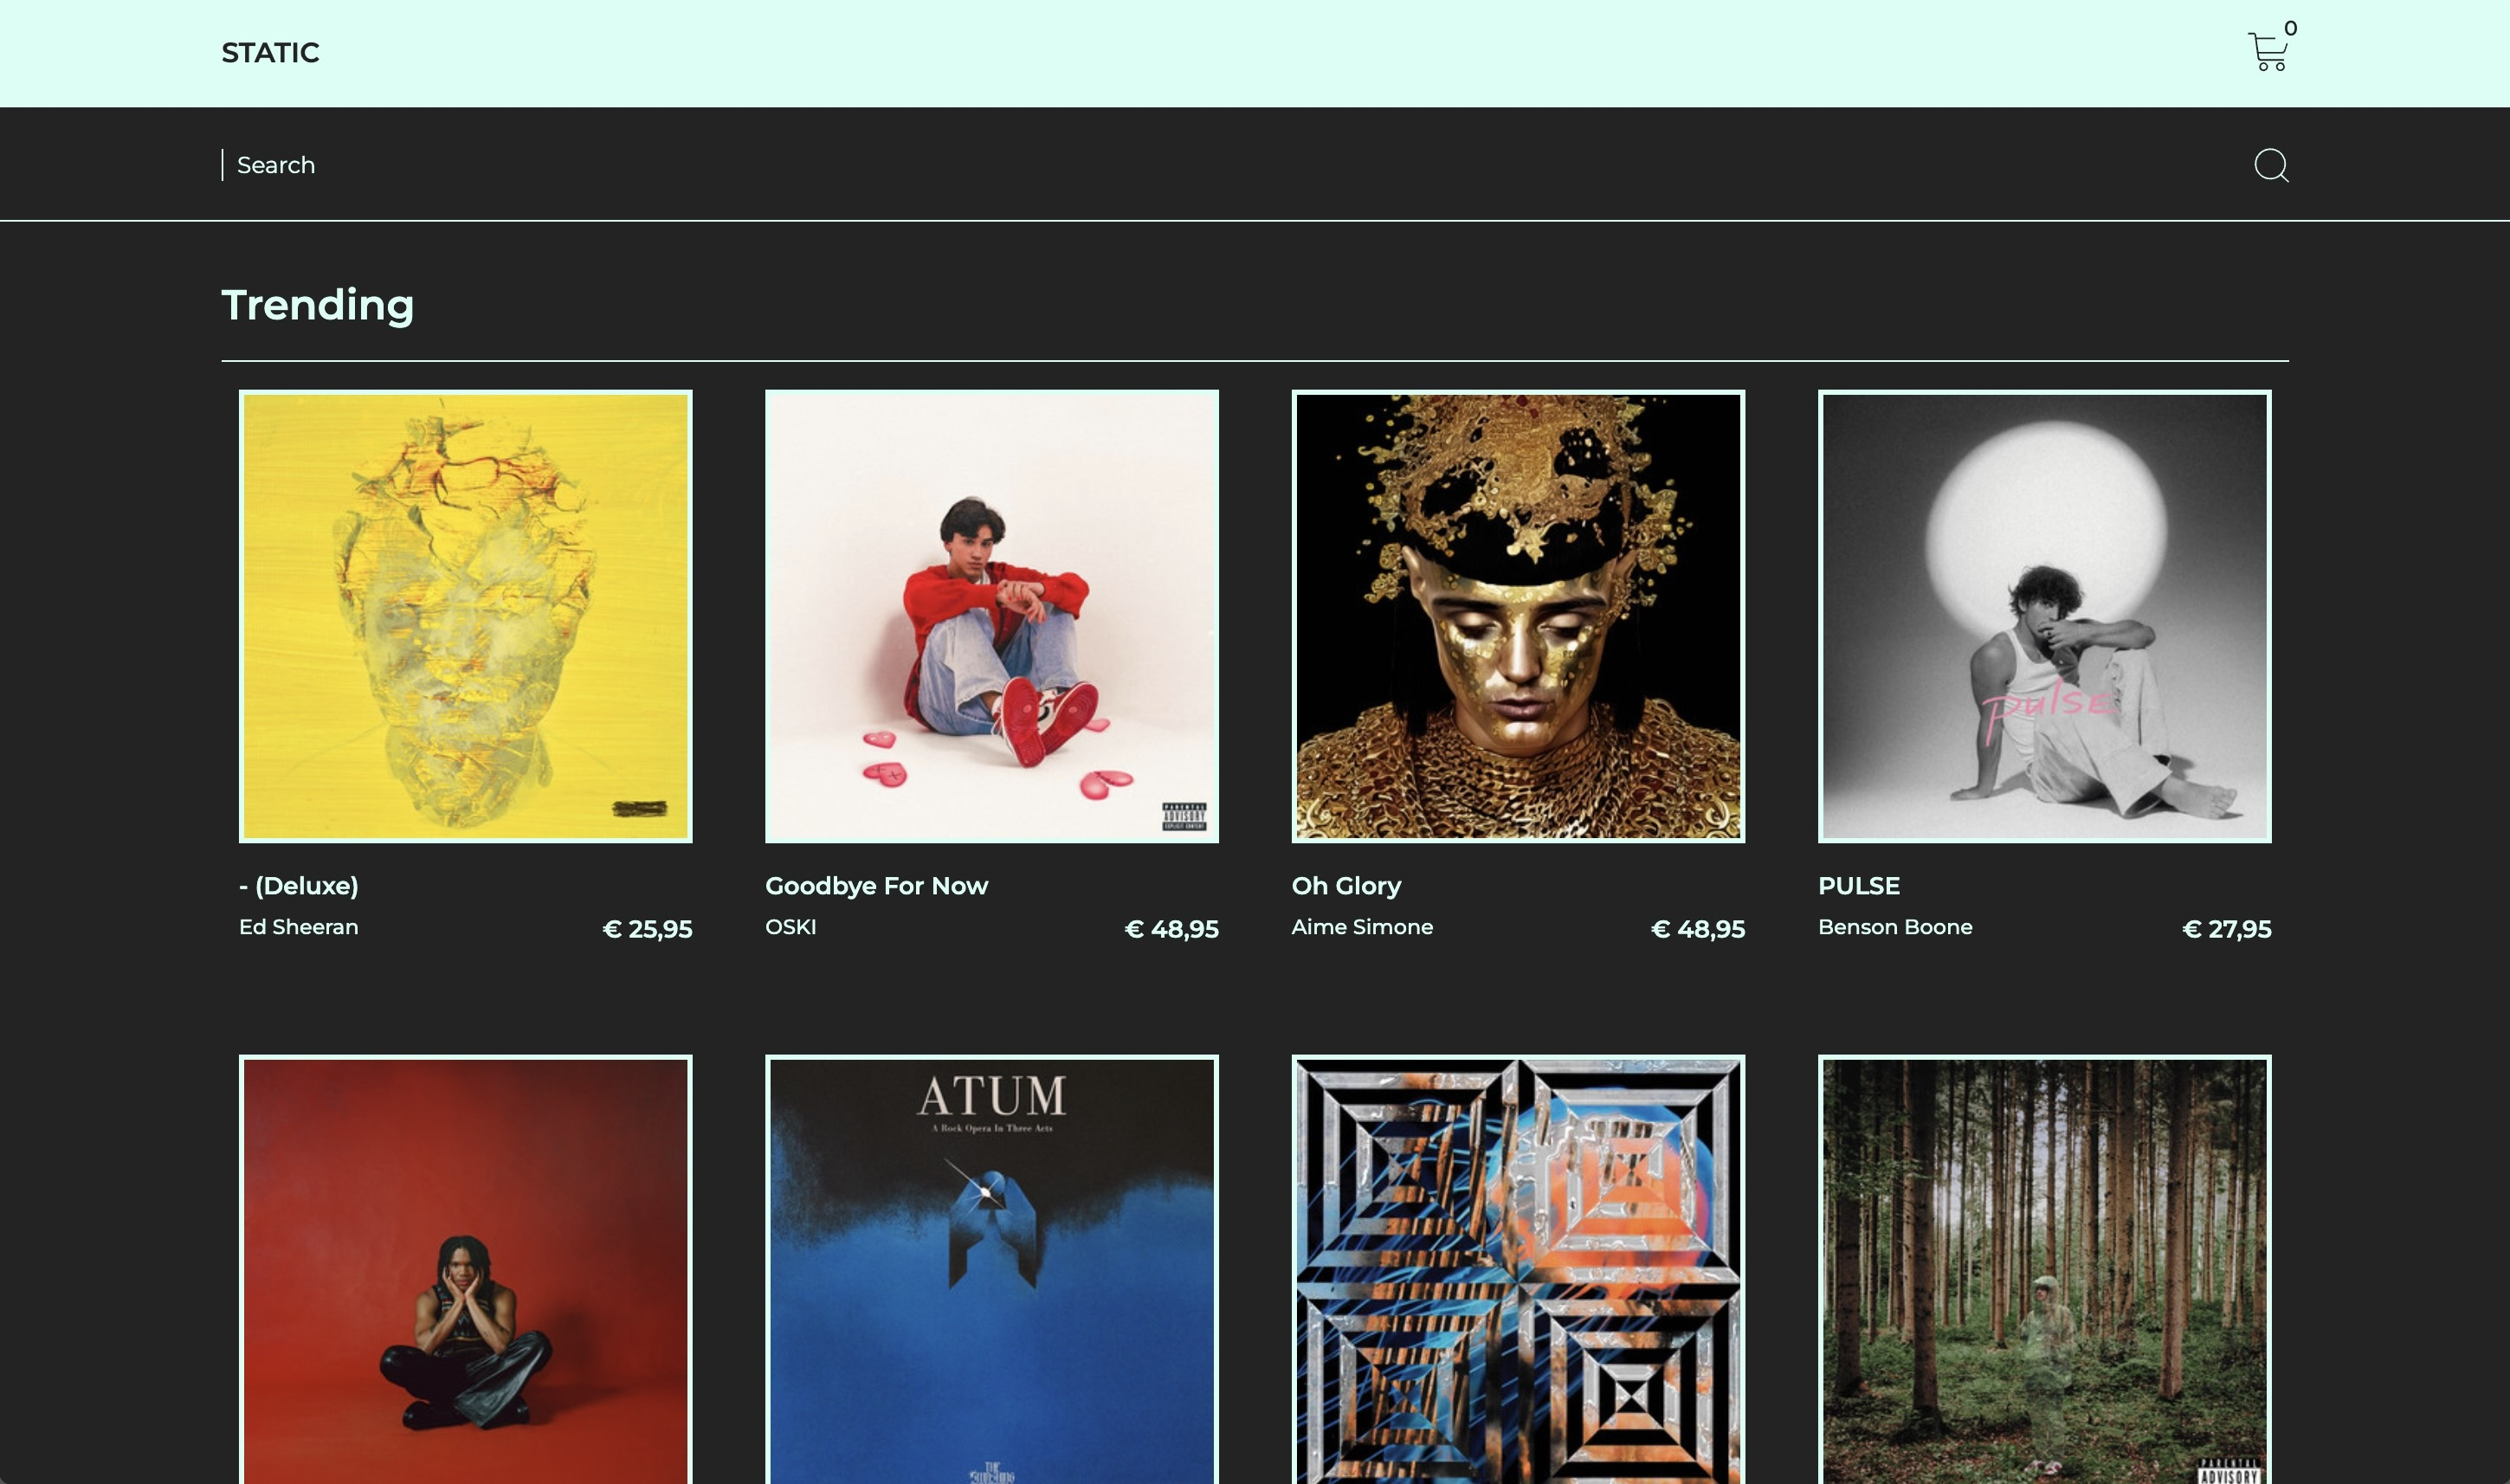
\includegraphics[width=1\linewidth]{graphics/desktopHomeConventioneel}
	\caption[Desktop home pagina conventioneel]{Desktop home pagina conventioneel}
	\label{fig:desktopHomeConventioneel}
\end{figure}

\newpage

\section{Detail pagina}

\subsection{Navigeren door de detail pagina}

Wanneer de gebruiker zich op de Detail pagina bevindt worden alle details getoond van de release. Waaronder de prijs, de releasedatum, het label en alle liedjes die behoren tot de release. De gebruiker heeft twee opties. Met de "ADD TO CART" knop kan men een release toevoegen aan de winkelmand of men kan ook doorverwezen worden naar Spotify om daar de release te beluisteren. Hier krijgt men ook opnieuw de mogelijkheid om naar een andere release te zoeken a.d.h.v. de zoekbalk. Als men een release toevoegt aan de winkelmand dan krijgt de gebruiker een pop-up ter bevestiging met twee opties, blijven door winkelen of naar de cart doorverwezen worden. Zie figuur \ref{fig:desktopDetailConventioneel} voor een beeld van de detail pagina.

\subsection{Hindernissen en uitdagingen}

Bij de detail pagina zijn weinig hindernissen opgetreden, een van de uitdagingen was om een 'GO BACK' knop te voorzien. Deze is nog op het laatste toegevoegd en vanuit een design perspectief dus niet het optimale moment. De knop bevindt zich nu in de header i.p.v. in vervanging van het logo als men naar een pagina gaat die niet de home pagina is. Wanneer een release toegevoegd wordt dan zal deze opgeslagen worden in de localStorage.

\begin{figure}
	\centering
	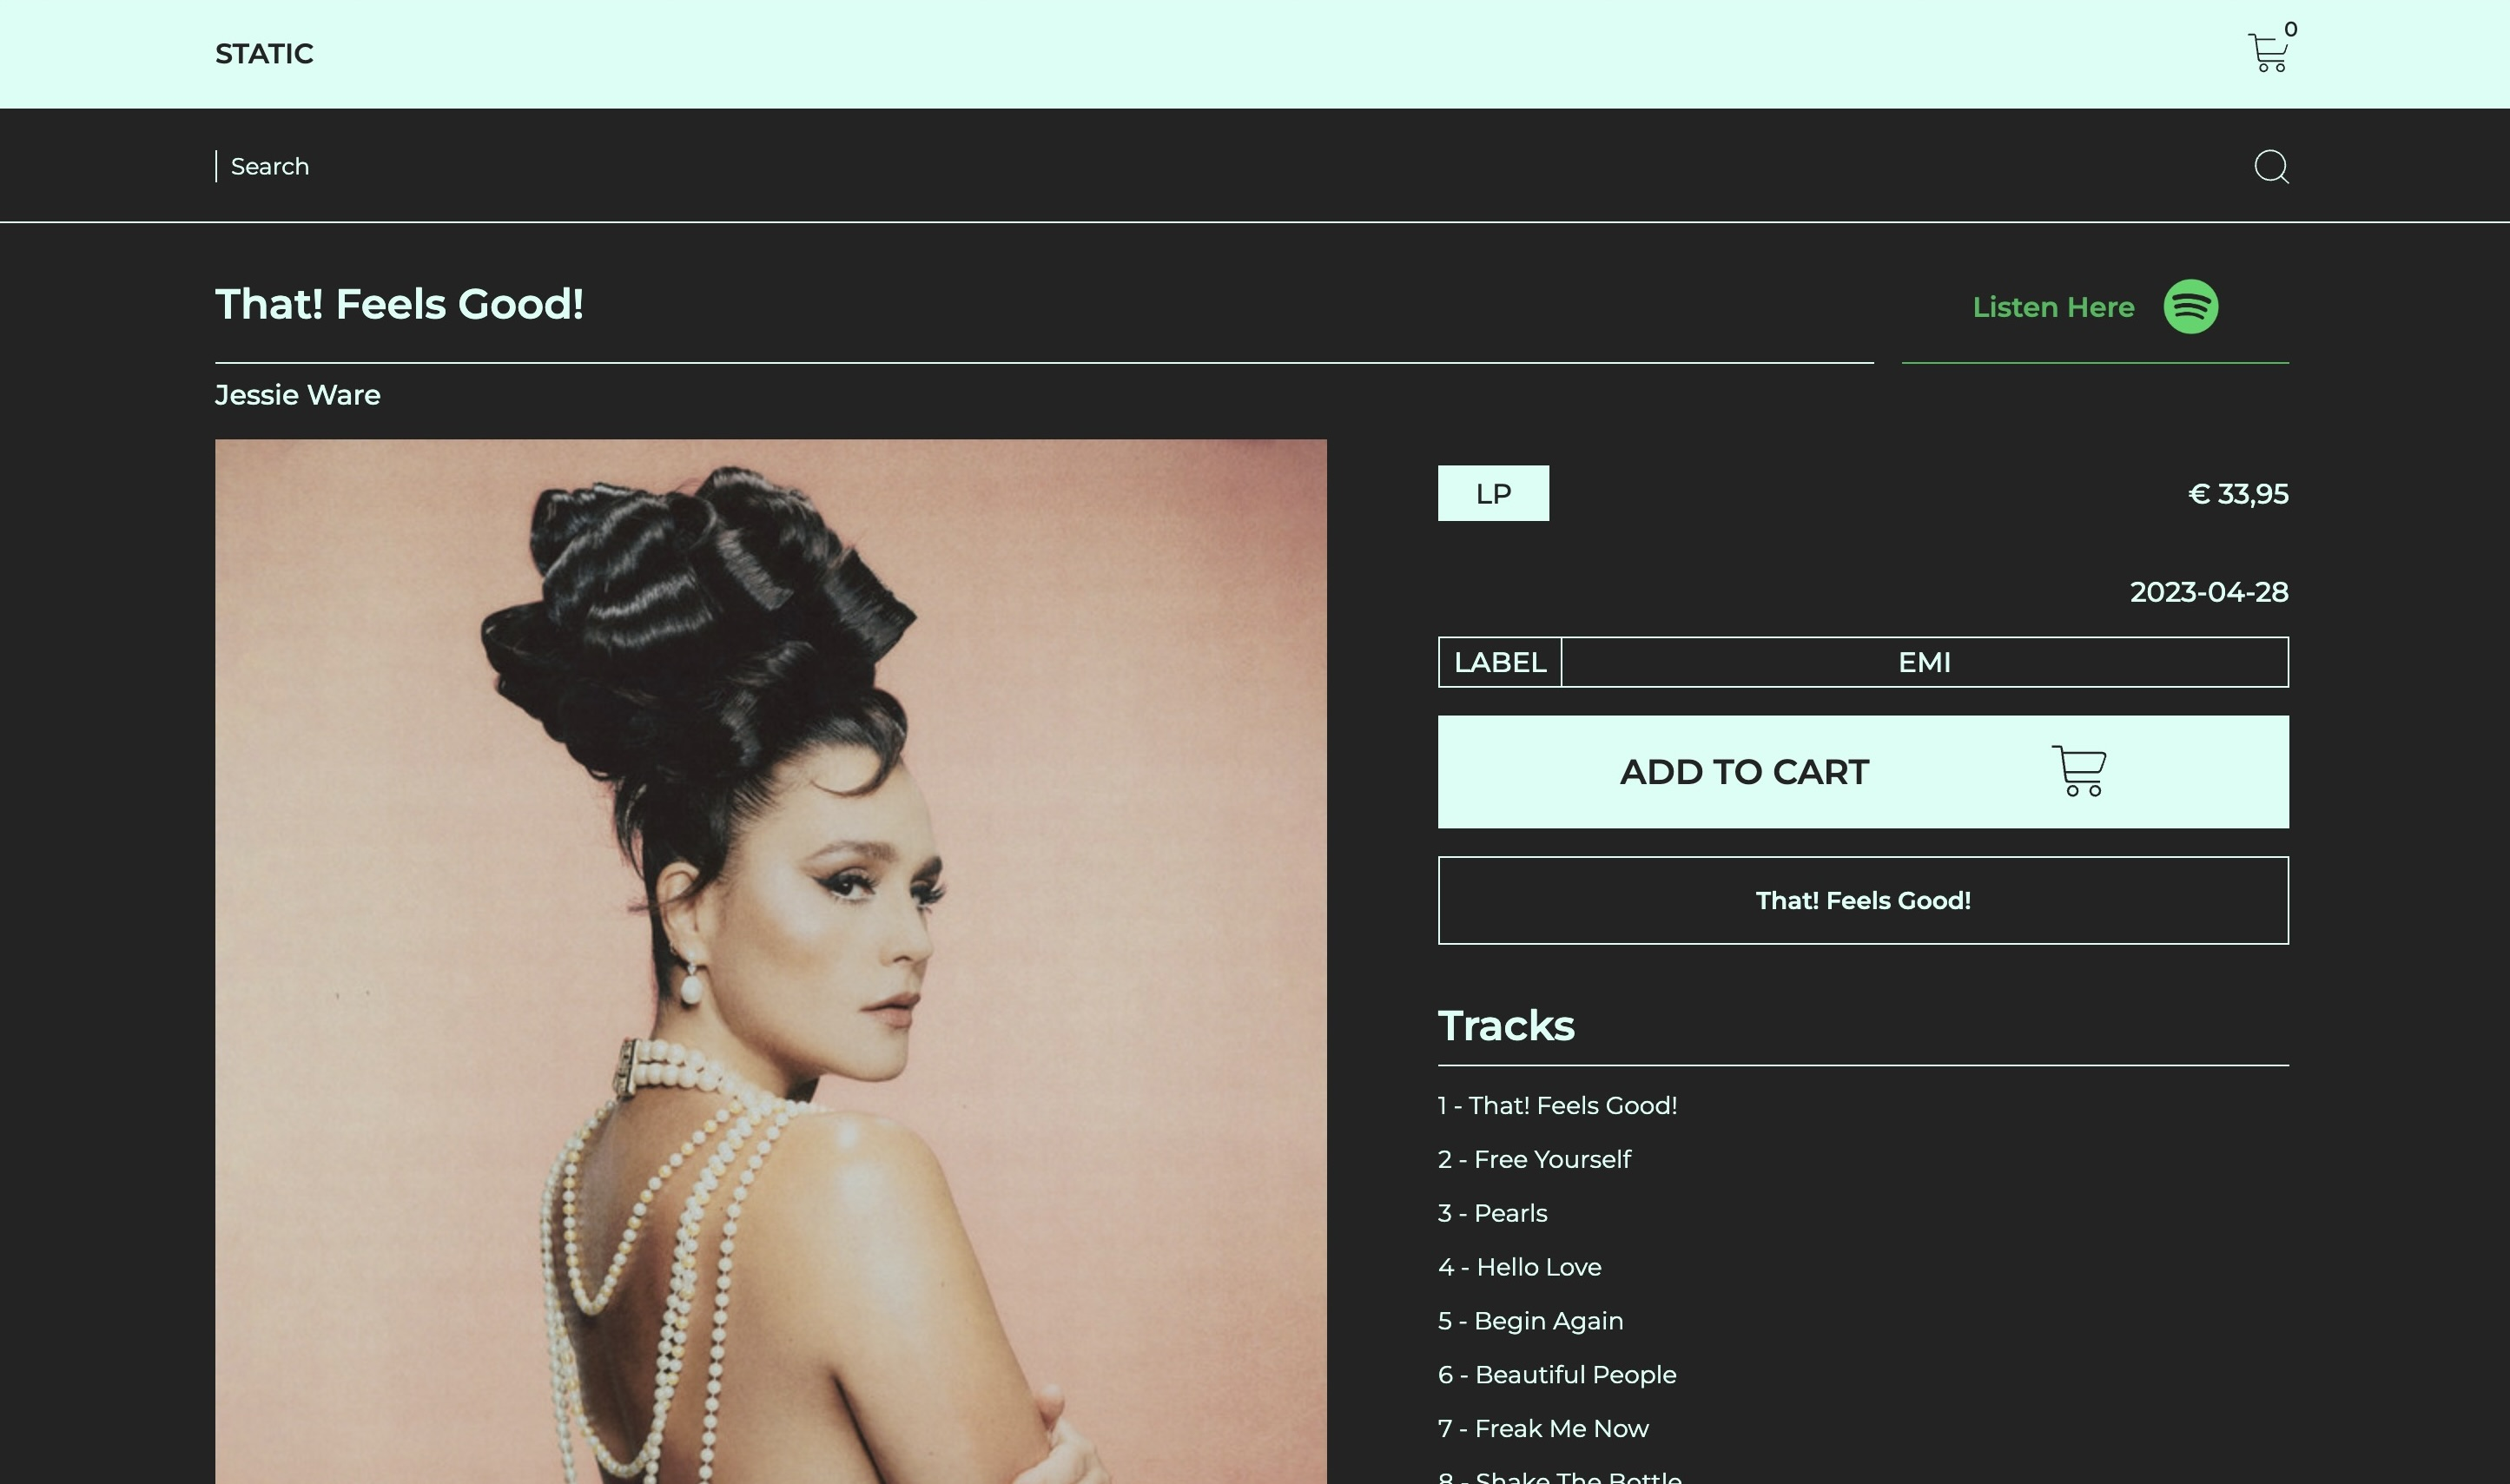
\includegraphics[width=1\linewidth]{graphics/desktopDetailConventioneel}
	\caption[Desktop detail pagina conventioneel]{Desktop detail pagina conventioneel}
	\label{fig:desktopDetailConventioneel}
\end{figure}

\section{Cart}

\subsection{Navigeren door de cart pagina}

Nu kan de gebruiker de geselecteerde releases bekijken in de winkelmand door in de header op het winkelmand icoon te klikken of bij het toevoegen aan de winkelmand op 'Go To Cart' te klikken. Hier krijgt men een overzicht van alle geselecteerde releases en kan men indien gewenst de hoeveelheid aanpassen of bepaalde releases verwijderen. Zie figuur \ref{fig:desktopCart} voor een beeld van de cart pagina.

\subsection{Componenten}

\subsubsection{Cart}

De Cart component haalt alle cartItems op uit de localStorage waar het id van de release wordt bijgehouden samen met de kwantiteit en prijs. Hierna worden een aantal calculaties uitgevoerd zijnde het berekenen van het aantal items in de cart samen met de totale prijs om de gebruiker een duidelijk overzicht te geven van de order. Voor elk item wordt een CartItem component aangemaakt en indien er geen items zijn dan word een gepaste boodschap getoond.

\subsubsection{CartItem}

Een CartItem bestaat uit de afbeelding en naam van de release, een dropdown keuzevak waarbij de kwantiteit kan veranderd worden indien gewenst, een 'Remove' knop en de individuele prijs van het item.

\begin{figure}
	\centering
	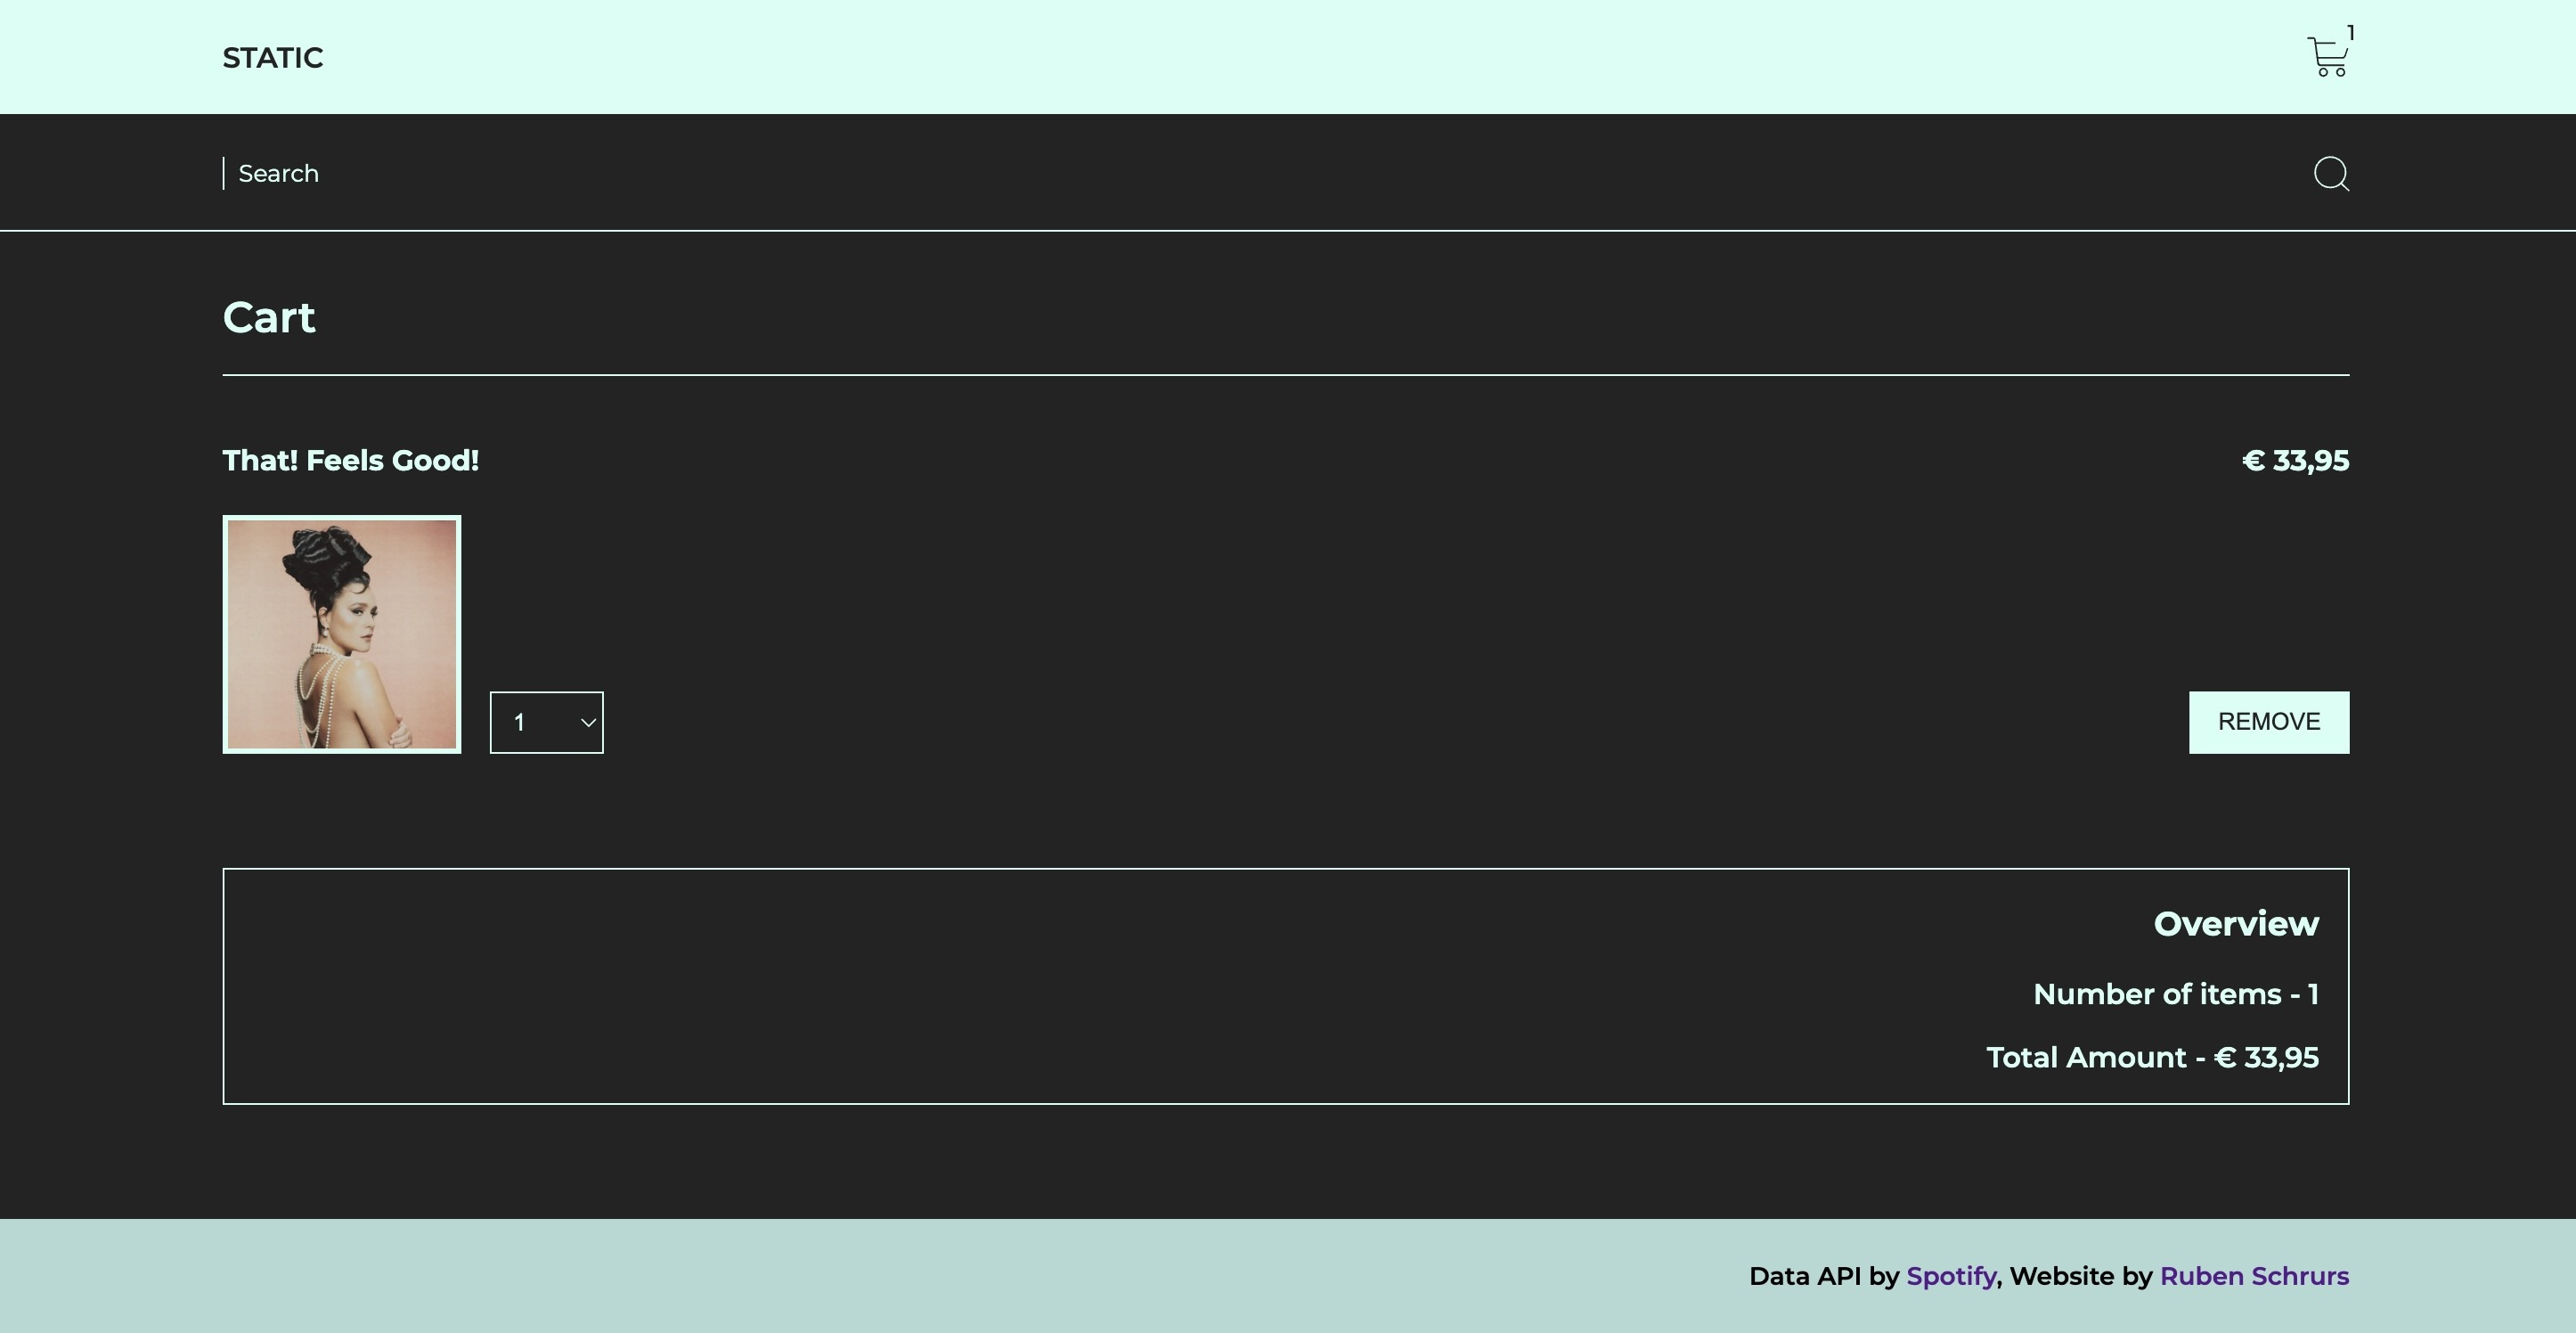
\includegraphics[width=1\linewidth]{graphics/desktopCart}
	\caption[Desktop cart pagina]{Desktop cart pagina}
	\label{fig:desktopCart}
\end{figure}

\section{Search}

Onder de header bevindt zich de search bar, deze kan de gebruiker over de volledige website gebruiken en zal volgend resultaat opleveren, zie figuur \ref{fig:desktopSearch}. De resultaten kunnen verborgen worden a.d.h.v. een 'Clear' knop rechts boven. De search bar maakt gebruik van de ReleaseItem component 

\subsection{Hindernissen en uitdagingen}

Een van de uitdagingen was om een prijs te genereren voor elk ReleaseItem wanneer de gebruiker een zoek query uitvoert. Hiernaast worden enkel resultaten getoond als er twee of meer karakters zijn in de query van de gebruiker, de reden hiervoor is om minder API calls uit te voeren.

\begin{figure}
	\centering
	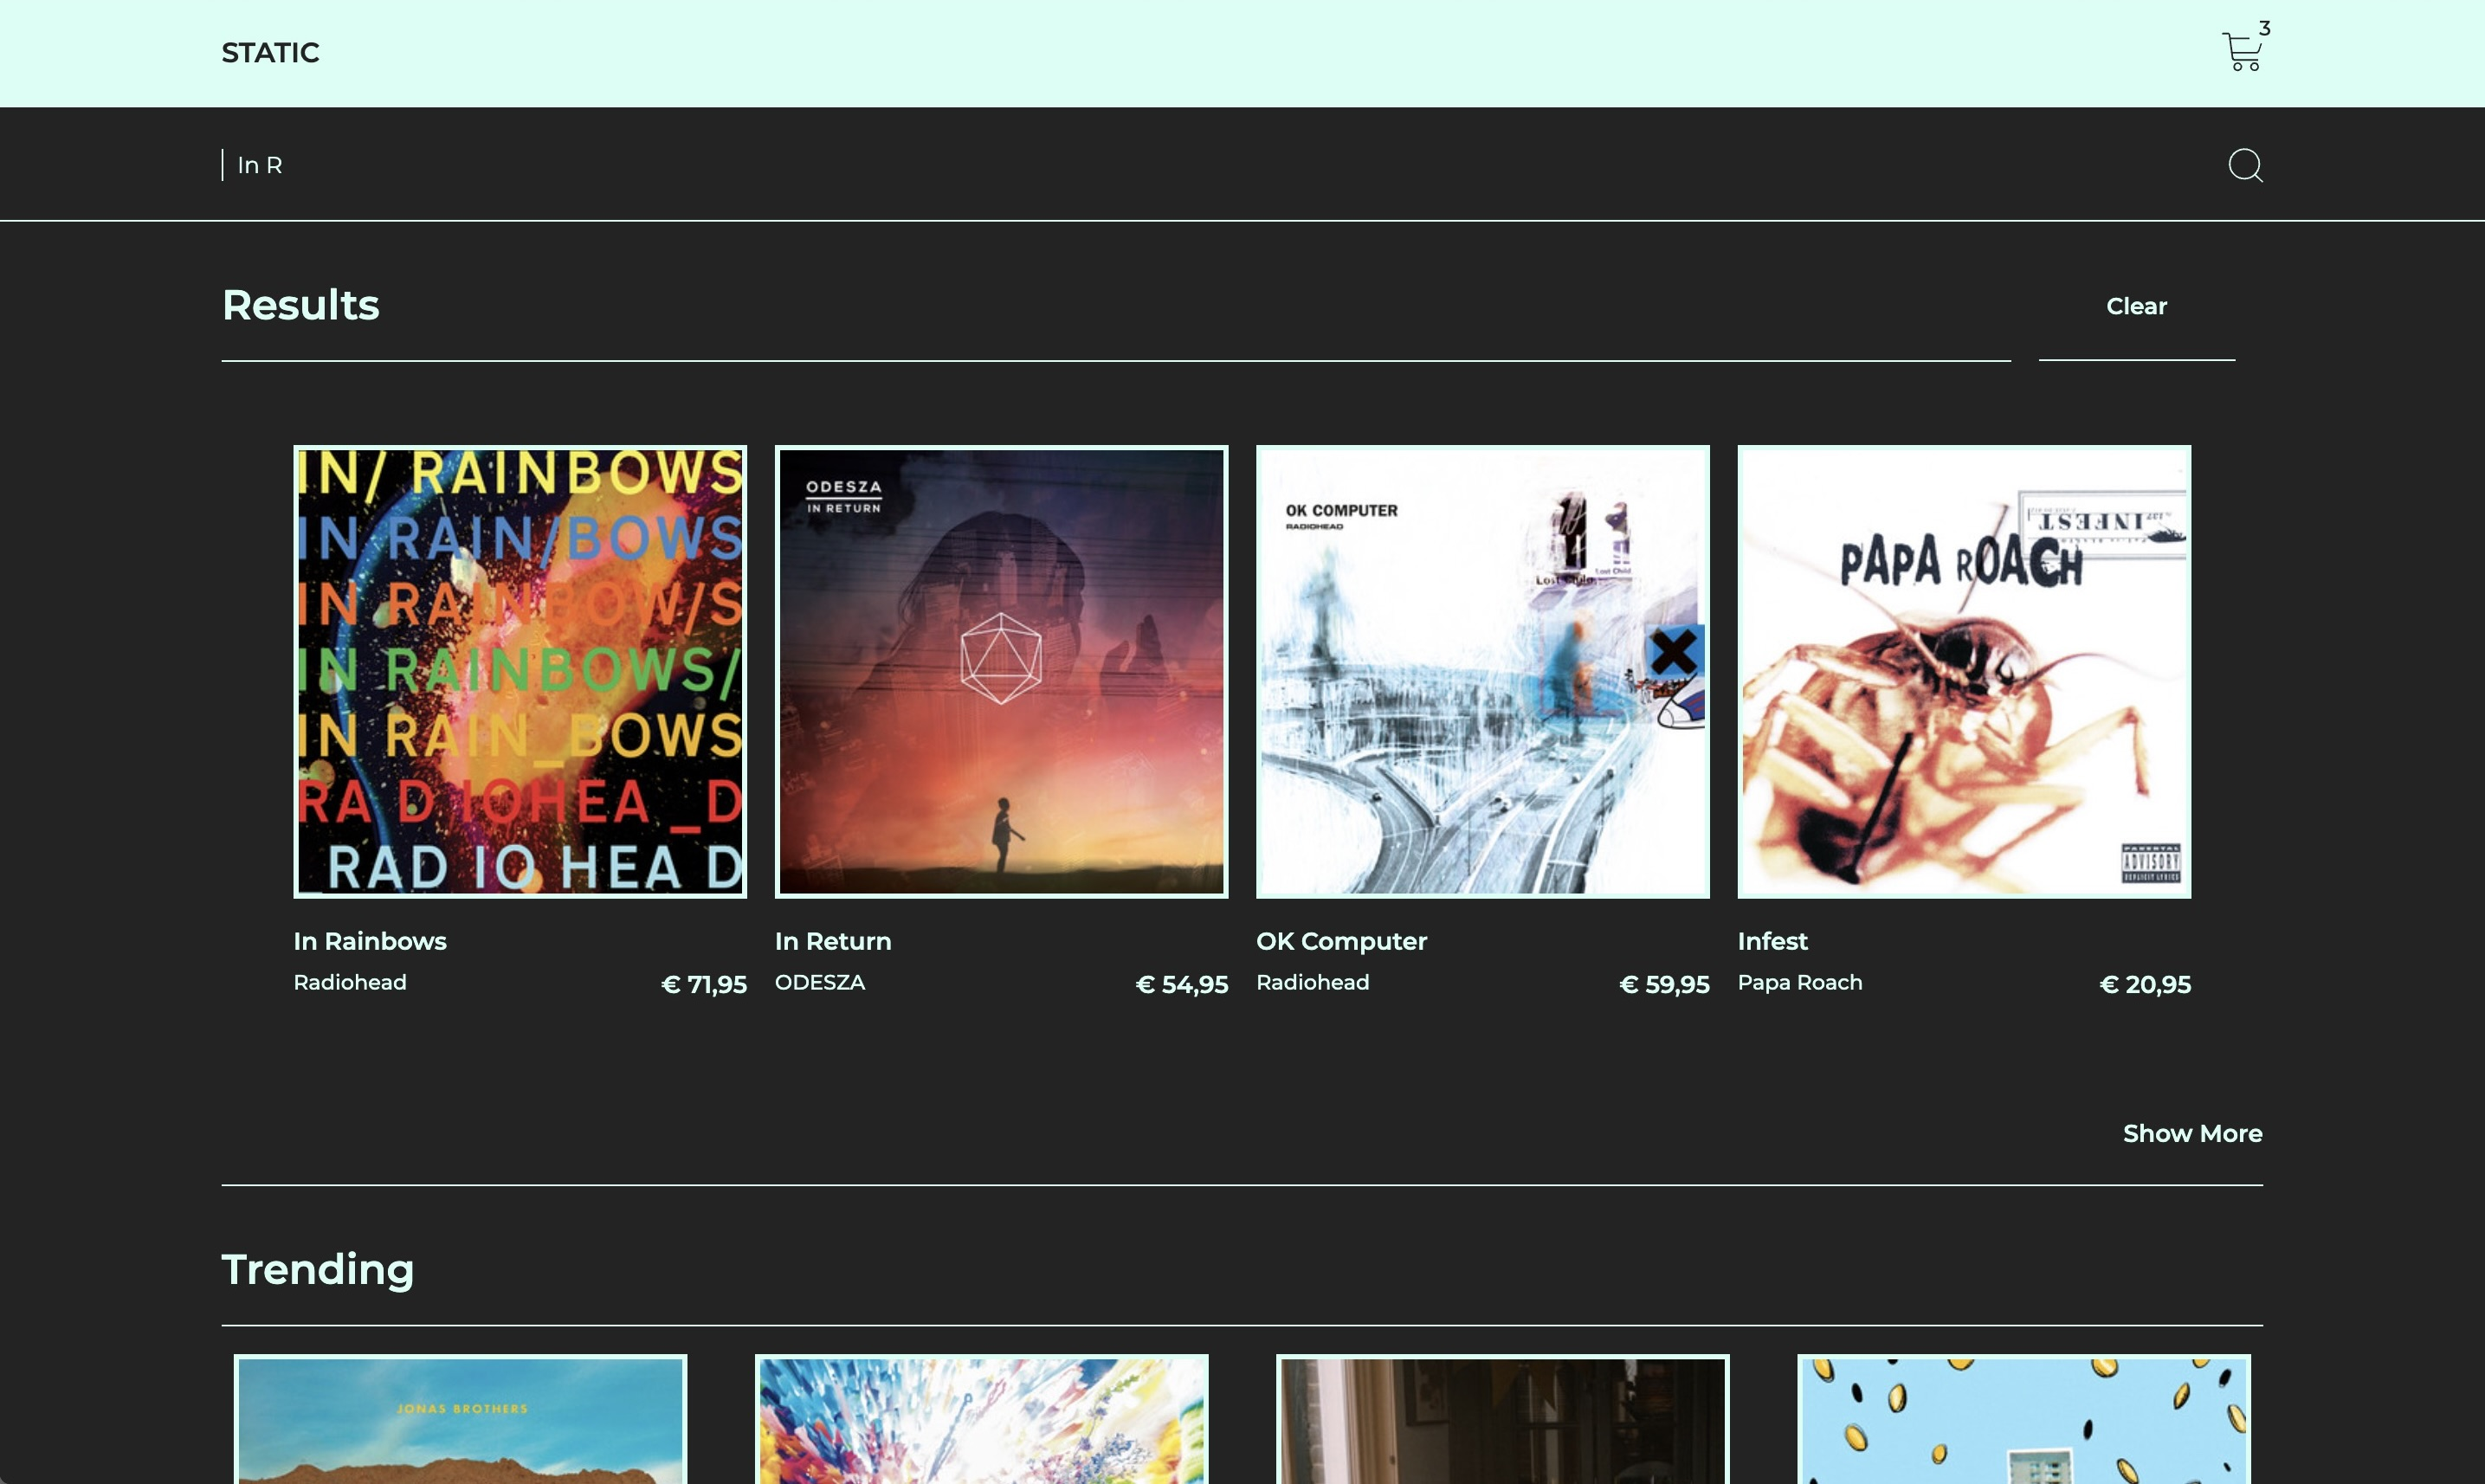
\includegraphics[width=1\linewidth]{graphics/desktopSearch}
	\caption[Desktop search]{Desktop search}
	\label{fig:desktopSearch}
\end{figure}

\section{Header}

De header bevindt zich uiteraard bovenaan en toont het logo en de cart met het aantal items in de cart. Als de gebruiker zich op de detail pagina of cart pagina bevindt dan wordt het logo vervangen door een 'GO BACK' knop.

\subsection{Hindernissen en uitdagingen}

Bij het tonen van het aantal items in de cart wordt een methode gebruikt die zich bevindt in de provider. Dit had een probleem opgelost waarbij de state van het aantal items niet geüpdatet werd ondanks er nieuwe items werden toegevoegd of de kwantiteit veranderd werd in de cart.
%%=============================================================================
%% Proof-of-concept: Three.js
%%=============================================================================

\chapter{\IfLanguageName{dutch}{Proof-of-concept: Three.js}{Proof-of-concept: Three.js}}%
\label{ch:proofofconceptThreeJS}

\section{Inleiding}

In dit hoofdstuk zal overlopen worden welke aanpassingen gemaakt zijn aan de conventionele POC. Hierbij zal een kijk genomen worden in hoe deze elementen opgebouwd zijn en welke voordelen ze met zich meebrengen.

Er zijn op twee plaatsen in de webshop aanpassingen gemaakt en dat is op de home pagina en de detail pagina. Voor de implementatie van de componenten is de React Three Fiber bibliotheek gebruikt.

\section{Home pagina}

Voor de home pagina zijn verschillende opties overwogen en uiteindelijk is gekozen voor een interactieve carrousel. Hierbij worden de releases naast elkaar weergegeven zodat de gebruiker intuïtief door de releases kan scrollen.

Onderaan de pagina bevindt zich een minimap die de positie van de gebruiker op de carrousel aangeeft.

De beide componenten bevinden zich in een \texttt{Canvas} die zich over de breedte van de volledige home pagina strekt. Het \texttt{Canvas} is als volgt geïnitialiseerd a.d.h.v. React Three Fiber: 

\newpage

\begin{LVerbatim}
<Canvas
	gl={{
			antialias: true,
			toneMapping: THREE.ACESFilmicToneMapping,
			outputEncoding: THREE.sRGBEncoding
	}}
	camera={{ position: [0, 0, 250] }}
	className='canvas'
>
	<HomeScene releases={newReleases?.albums?.items}/>
</Canvas>
\end{LVerbatim}

Het \texttt{Canvas} krijgt standaard instellingen mee voor de renderer via de 'gl' property. De camera wordt ook 250 eenheden naar achter geplaatst zodat de objecten in de scene kunnen gezien worden. Binnen in het \texttt{Canvas} wordt een \texttt{HomeScene} component meegegeven met de nodige data voor het tonen van de releases.

\begin{figure}
	\centering
	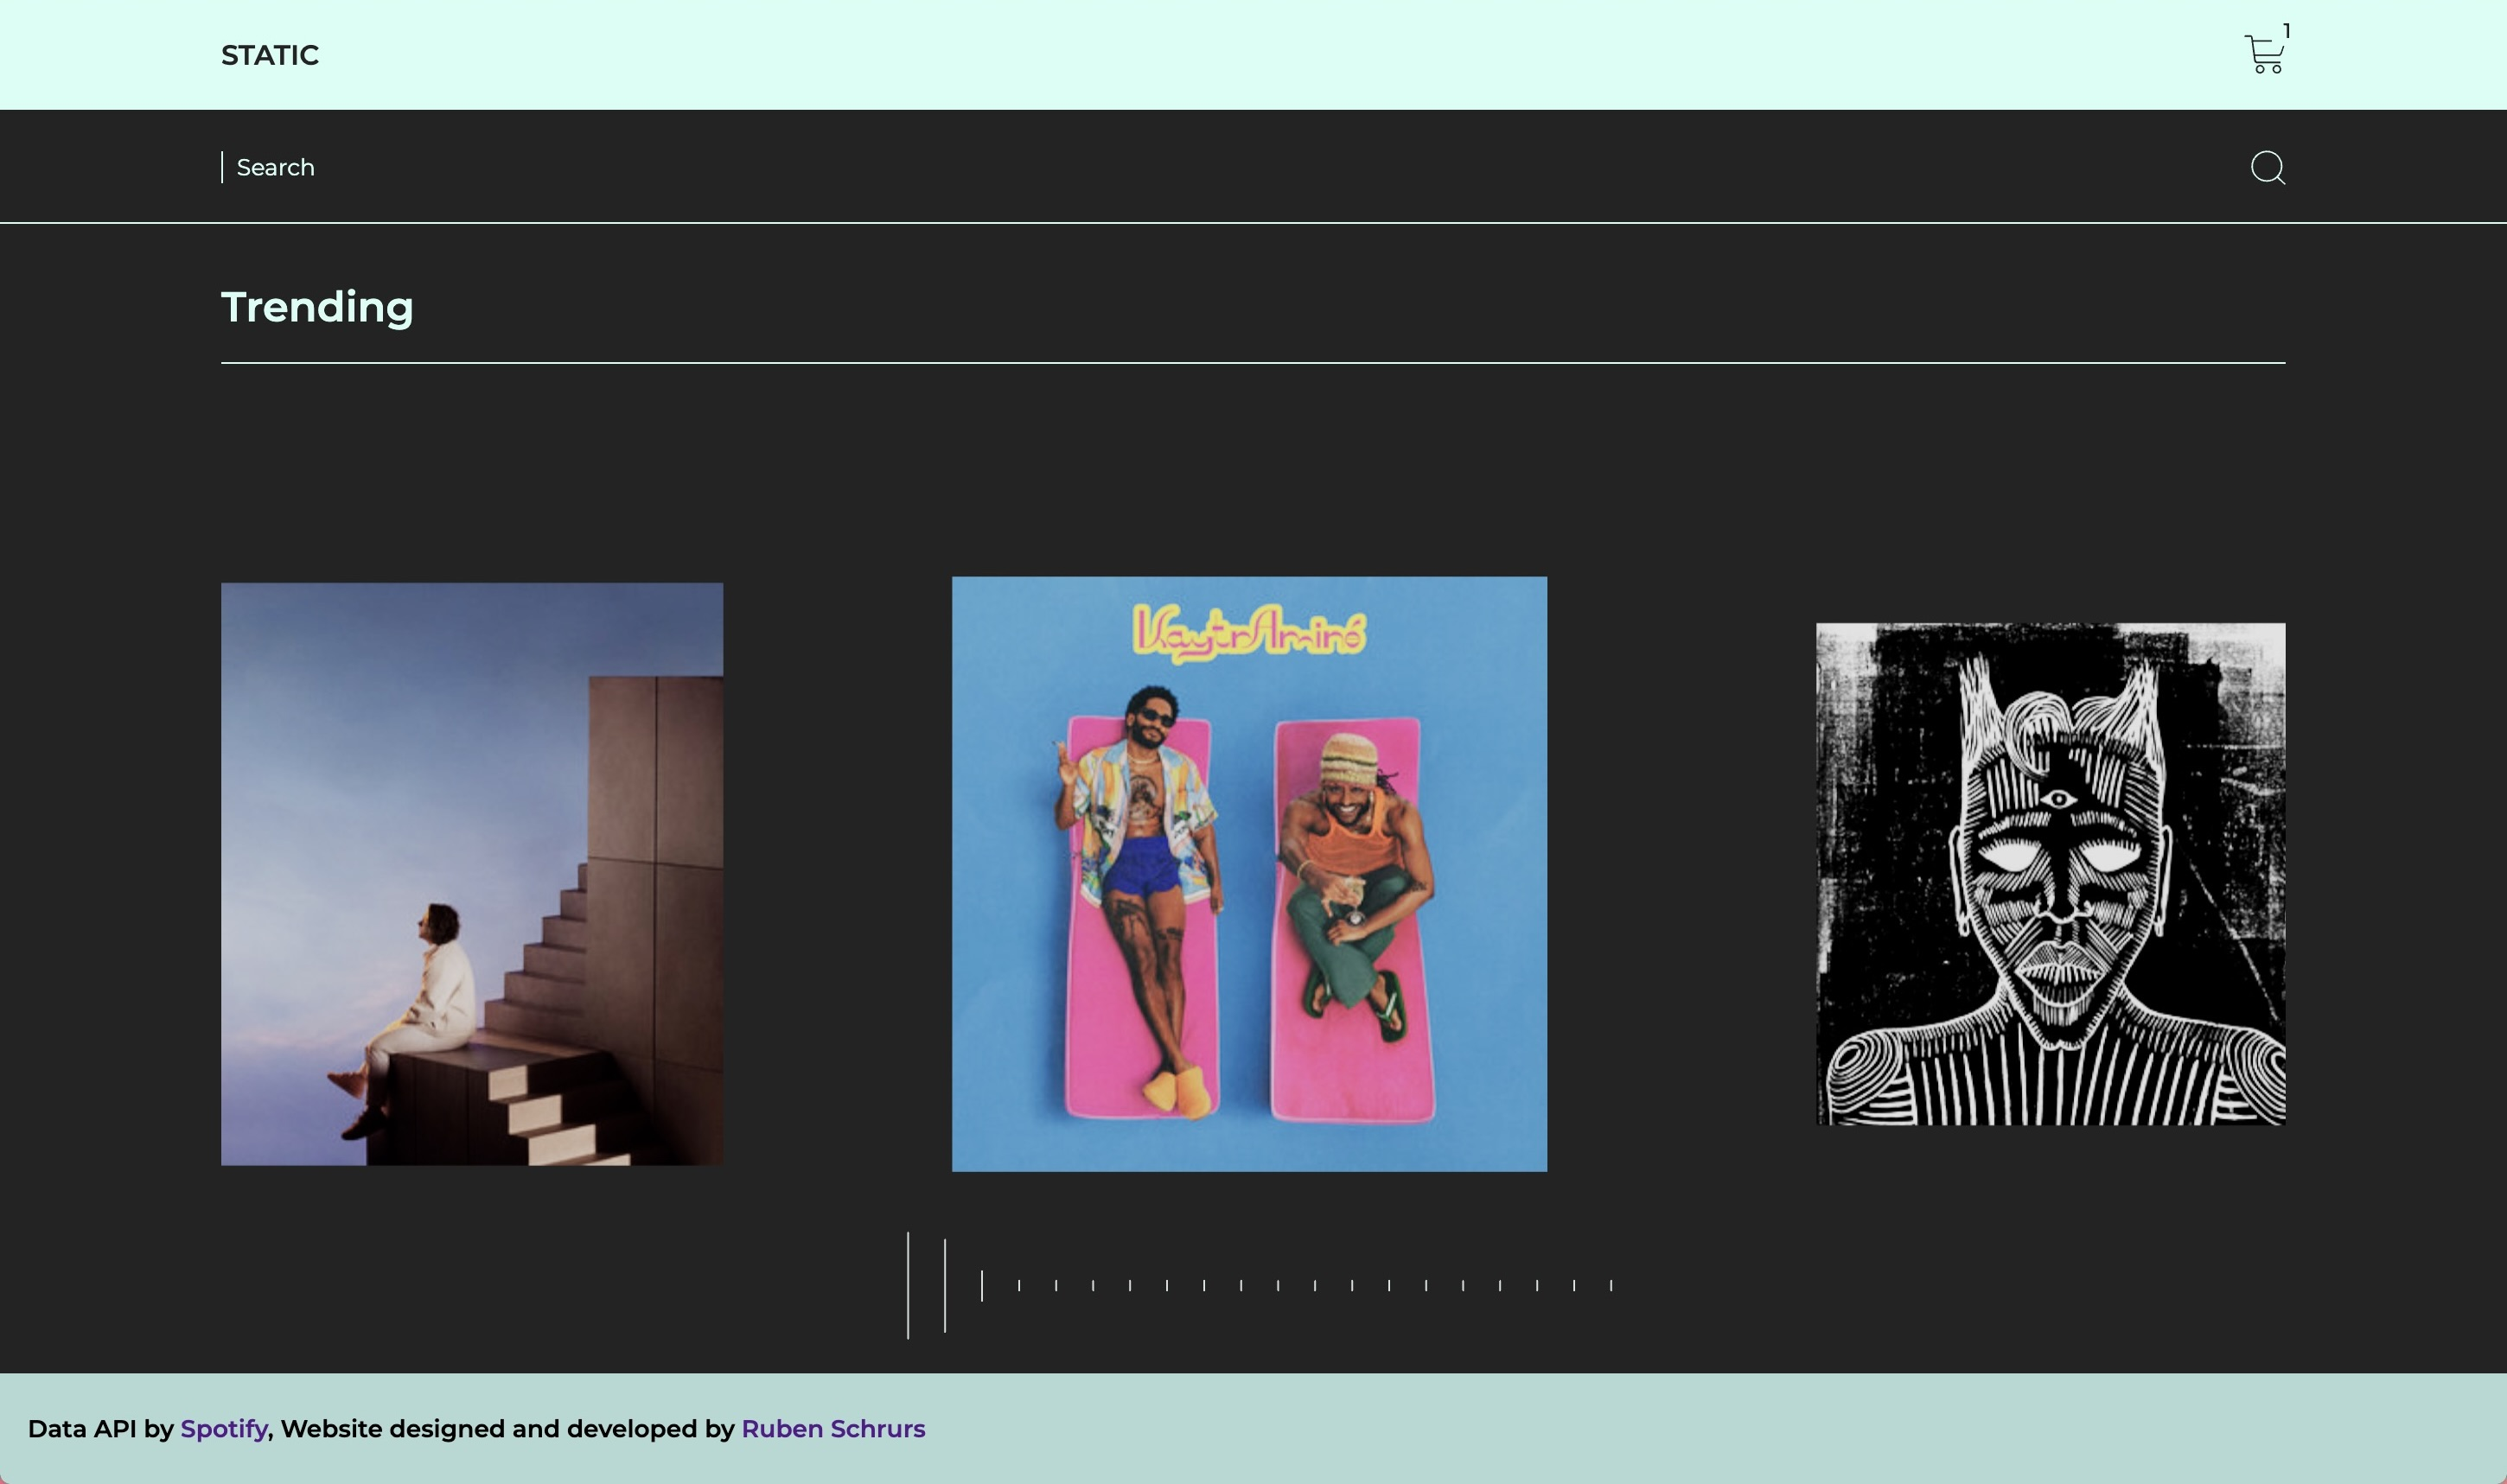
\includegraphics[width=1\linewidth]{graphics/desktopHomeThree}
	\caption[Home pagina Three.js]{Home pagina Three.js}
	\label{fig:desktopHomeThree}
\end{figure}

\newpage
\subsection{HomeScene}

In de \texttt{HomeScene} component worden alle vereiste gegevens doorgegeven om een scene te bouwen. Hieronder vindt u de code voor de renderfunctie van de \texttt{HomeScene}:
\newline
\newline
\begin{BVerbatim}
<directionalLight castShadow position={[0, 0, 1]} />
<ambientLight intensity={0.5} />
<ScrollControls
	pages={(width - xW + totalLength * xW) / width}
	horizontal={!isMobile}
	damping={0.1}
>
	<Scroll>
		<Suspense fallback={<Placeholder position-y={1} scale={[20, 20, 20]} />}>
			<group>
			{
				releases?.map((release, index) => {
					return (
						<ReleaseItem3D
							key={index}
							index={index}
							position={[
								index * xW,
								0, 0
								]}
							scale={scale}
							setScale={setScale}
							release={release}
							totalLength={totalLength}
						/>
					)
				})
			}
			</group>
		</Suspense>
	</Scroll>
	<Minimap items={releases} />
</ScrollControls>
\end{BVerbatim}
\newpage

Als eerste wordt een directioneel licht object meegegeven met de volgende props:

\begin{itemize}
	\item castShadow
	\item position={[0, 0, 1]}
\end{itemize}

De \texttt{castShadow} prop is vanzelfsprekend en zorgt er dus voor dat dit licht object de mogelijkheid krijgt om schaduwen de produceren. De positie van het licht ligt niet in het centrum van de scene omdat de 3D tekst anders moeilijker zichtbaar is. Dit soort licht zal ervoor zorgen dat alle objecten in de scene even belicht zijn vanuit dezelfde richting.

Het volgende licht is een omgevingslicht of \texttt{AmbientLight} object, dit licht zorgt ervoor dat alle vlakken van de 3D tekst zichtbaar zijn. De intensiteit is lager dan de normaal waarde voor een gevoel van perspectief te creëren.

\texttt{ScrollControls} is een van de componenten die beschikbaar wordt gesteld door de bibliotheek react-three/drei. Voor deze component geef je het aantal pagina's door, hiervoor wordt een berekening uitgevoerd op basis van de breedte van de viewport, de lengte van het aantal weergegeven items, en de breedte van elk item plus de opening of 'gap' tussen elk item. De scroll richting kan ook bepaald worden en zal veranderen op basis van de breedte van de viewport. De laatste prop is de 'damping' die bepaald in welke mate de scrollbeweging gedempt wordt.

Alle 3D objecten waardoor gescrolld moet worden worden binnen in een \texttt{Scroll} component geplaatst.

\subsubsection{Carrousel}

In de \texttt{Scroll} component wordt \texttt{Suspense} gebruikt, een native react component, die een fallback zal tonen terwijl de objecten worden ingeladen. In dit geval is dat een \texttt{Placeholder} component die een simpele \texttt{BoxGeometry} is.

Er wordt vervolgens gemapt over de release items en voor elke item een \texttt{ReleaseItem3D} terug gegeven. Hierbij krijgt de component ook de nodige info zoals de positie en schaal.

De \texttt{ReleaseItem3D} component heeft volgende renderfunctie:

\begin{BVerbatim}
<group ref={releaseContainer} position={position}>
	<Image 
		ref={releaseImage} 
		scale={scale} url={url} 
		onClick={handleReleaseItem} 
		onPointerOver={over} 
		onPointerOut={out} 
	/>
	{
		hovered ? (
			<group>
				<mesh ref={titleRef} position={[-150, 150, 0]}>
					<textGeometry 
						args={[
							releaseName,
							{ font, size: 15, height: 1 }
						]} 
					/>
					<meshPhysicalMaterial 
						attach='material' 
						color={App.secondaryColor} 
					/>
				</mesh>
				<mesh position={[100, 150, 0]}>
					<textGeometry 
						args={[
							`€ ${price}`,
							{ font, size: 12, height: 1 }
						]} 
					/>
					<meshPhysicalMaterial 
						attach='material' 
						color={App.secondaryColor} 
					/>
				</mesh>
			</group>
		) : (
			null
		)
	}
</group>
\end{BVerbatim}

De objecten worden genest in een \texttt{<group>} tag, dit is verplicht bij het gebruik van meerdere R3F componenten en wordt ook gebruikt om de positie van het volledige object te bepalen.
De \texttt{Image} component is een \texttt{react-three/drei} abstractie en krijgt een gepaste schaal mee die afgestemd is op de grootte van de scene alsook de url voor de afbeelding. Wanneer er geklikt wordt op de component dan zal de gebruiker doorverwezen worden naar de detailpagina. Hiernaast wordt ook een boolean bijgehouden of de gebruiker al dan niet hovered over de afbeelding. Indien deze waarde op \texttt{true} komt te staan dan zullen twee 3D text objecten toegevoegd worden in de scene gepositioneerd boven de afbeelding. Linksboven de afbeelding is dat de naam van de release en rechtsboven de prijs, wanneer de naam van de release te lang is dan zal de string waarde afgekapt wordt een beletselteken ingevoegd.

De \texttt{ReleaseItem3D} component bevat een \texttt{useFrame} hook die voor elke frame een nieuwe render zal uitvoeren. 
\newline

\begin{BVerbatim}
const scroll = useScroll()

useFrame((state, delta) => {
	const y = scroll.curve(index / totalLength - 1.5 / totalLength, 4 / totalLength)
	
	if (hovered) releaseImage.current.scale.x = damp(
		releaseImage.current.scale.x, 300, 6, delta
	)
	if (hovered) releaseImage.current.scale.y = damp(
		releaseImage.current.scale.y, 300, 6, delta
	)
	
	releaseImage.current.scale[0] = releaseImage.current.scale.x = damp(
		releaseImage.current.scale.x, scale[0] * .6 + scrollValue * 75, 8, delta
	)
	releaseImage.current.scale[1] = releaseImage.current.scale.y = damp(
		releaseImage.current.scale.y, scale[1] * .6 + scrollValue * 75, 8, delta
	)
})
\end{BVerbatim}

Op de eerste lijn wordt een \texttt{scrollValue} variabele gedefinieerd die een waarde krijgt op basis van de curve functie van de \texttt{useScroll()} hook. Deze variabele bepaald hoe ver de component ligt t.o.v. het midden waarbij \texttt{scrollValue = 1} als absoluut midden van de scene kan gezien worden. Als de \texttt{hovered} boolean \texttt{true} is dan wordt een animatie uitgevoerd en verandered de schaal van de afbeelding, zie figuur \ref{fig:desktopHomeThreeHovered}. Vervolgens gebruiken we de \texttt{scrollValue} variabele om de schaal van de afbeelding aan te passen wanneer de \texttt{hovered} boolean opnieuw \texttt{false} is, zo keert de schaal terug naar de originele staat. 
Voor beide transformaties wordt gebruik gemaakt van de \texttt{damp()} functie, deze maakt deel uit van het \texttt{MathUtils} object uit de Three.js bibliotheek. De functie zal vloeiend een getal interpoleren van x naar y op een veerachtige manier, dat komt doordat gebruik gemaakt wordt van \texttt{delta} om de beweging onafhankelijk te houden van de beeldsnelheid. De eerste parameter is het startpunt en tweede de doelwaarde, als derde komt de lambda waarde die de snelheid van de veerkracht bepaald waarbij een hogere waarde een snellere transitie zal voortbrengen.

\begin{figure}
	\centering
	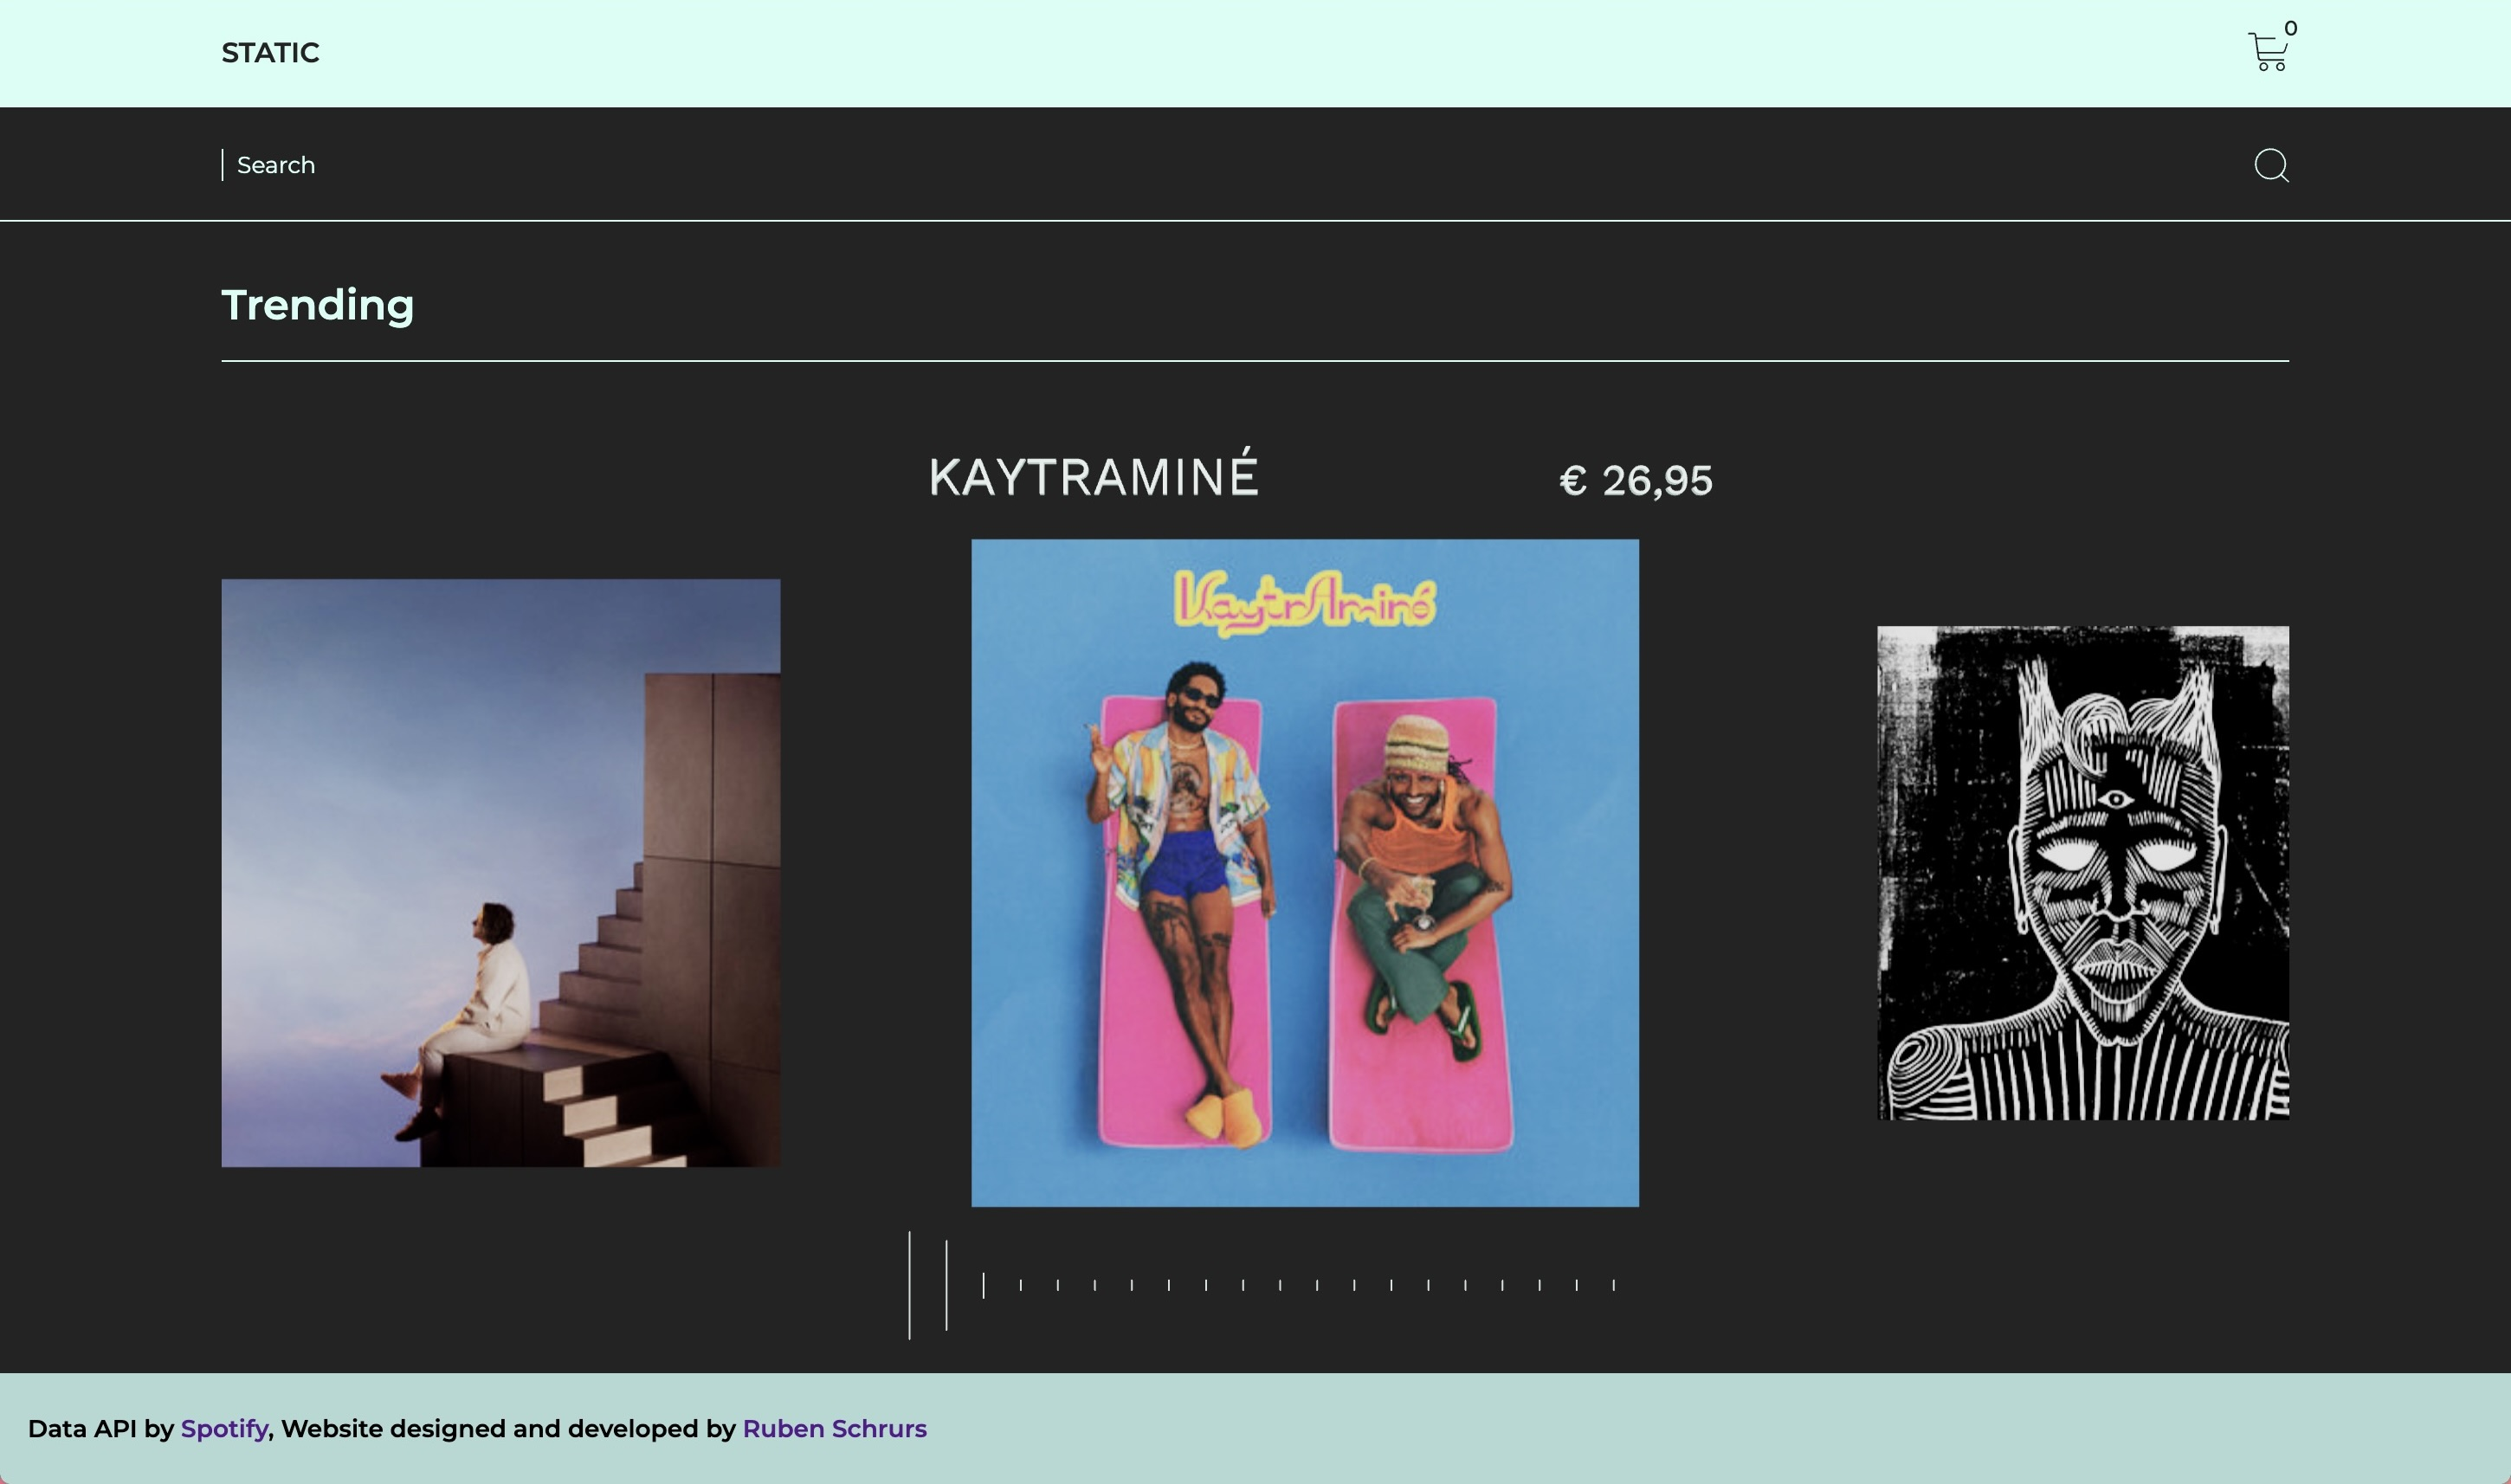
\includegraphics[width=1\linewidth]{graphics/desktopHomeThreeHovered}
	\caption[Home pagina Three.js hovered]{Home pagina Three.js hovered}
	\label{fig:desktopHomeThreeHovered}
\end{figure}

\subsubsection{Minimap}

De \texttt{Minimap} component geeft de gebruiker een overzicht over waar die zich bevindt in de carrousel. Dit is gedaan a.d.h.v. verticale lijnen die naast elkaar geplaatst worden. De renderfunctie voor de \texttt{Minimap} component is de volgende: 

\begin{figure}
	\centering
	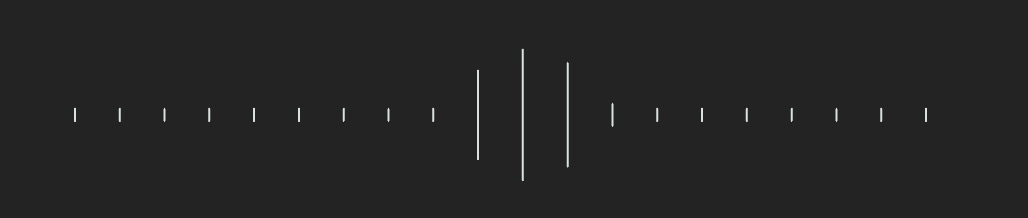
\includegraphics[width=1\linewidth]{graphics/minimap}
	\caption[Minimap]{Minimap}
	\label{fig:minimap}
\end{figure}

\begin{BVerbatim}
return (
	<group ref={minimapRef}>
		{items?.map((_, i) => (
			<group 
				key={i} 
				position={[
					i * 15 - items.length * 7,
					- height / 2 + 25,
					-5
				]}
			>
				<Line 
					points={[
						new THREE.Vector3(0, -20, 0),
						new THREE.Vector3(0, 20, 0)
					]} 
					color={App.secondaryColor} 
					lineWidth={1}
				/>
			</group>
			))}
	</group>
)
\end{BVerbatim}
\newline
\newline
Er wordt over de items gemapt die zijn meegegeven aan de \texttt{Minimap} en voor elk item een \texttt{Line} component gegenereerd. De \texttt{Line} bestaat uit twee \texttt{Vector3} objecten en zal tussen deze twee objecten een lijn tekenen met de meegegeven kleur en dikte. Elke lijn krijgt een positie die gebaseerd is op de lengte van het aantal items en de hoogte van de viewport.
Nu alle lijnen gerenderd zijn wordt er ook elke frame een nieuwe render gedaan a.d.h.v. de volgende \texttt{useFrame} hook.
\newline
\newline
\begin{BVerbatim}
useFrame((state, delta) => {
	minimapRef.current.children.forEach((child, index) => {
		const y = scroll.curve(
			index / items.length - 0.15 / items.length,
			4 / items.length
		)s
		child.scale.y = damp(child.scale.y, .1 + y, .8, .2, delta)
	})
})
\end{BVerbatim}

In deze useFrame wordt voor elke lijn van de minimap een \texttt{y} variabele gemaakt op basis van het aantal lijnen en de plaats van de individuele lijn. Vervolgens gebruiken we deze om de schaal van de lijn aan te passen met de \texttt{damp()} functie. Deze transformaties zorgen ervoor dat een golf effect over de lijnen wordt geplaatst wanneer de gebruiker scrollt, zie fig. \ref{fig:minimap}.

\subsection{Hindernissen en uitdagingen}

Het originele idee was om een platenhoes en vinyl plaat in 3D te modelleren en deze dan te importeren in de scene. Dit bleek echter zeer tijdrovend zeker voor een beginner in 3D modelleren. Alhoewel het gelukt is om een platenhoes te modelleren was dat niet het geval voor het plaatsen van een afbeelding op het 3D model. Een van de redenen was omdat het model over meerdere vlakken beschikte, na veel zoeken is dan uiteindelijk gekozen voor een \texttt{PlaneGeometry}. Deze oplossing werd dan opnieuw herzien en vervangen door de \texttt{Image} component uit de \texttt{react-three/drei} bibliotheek.

De 3D tekst is ook een aantal fases ondergaan. Een van de problemen was dat de font die gebruikt wordt over de gehele conventionele versie niet compatibel is. Er vond namelijk af en toe een glitch plaats bij een of meerdere van de letters of cijfers in de font. Niet alle fonts konden dus voor dit project gebruikt worden, na een aantal fonts te proberen is uiteindelijk gekozen voor \texttt{Work Sans Regular}.

\section{Detail pagina}

Het originele idee voor de detail pagina was om dezelfde scene te behouden en een animatie te voorzien om tussen de twee pagina's te wisselen. Na een aantal pogingen is toch gekozen voor een de oude scene te verwijderen en een nieuwe in te brengen wanneer een gebruiker op een item klikt.

De hoofdtitel van de detail pagina is dezelfde als de conventionele en bevat ook een link naar de spotify URL voor de release. Verder bevind zich op de linkerhelft van de pagina een 3D representatie van de album cover met een \texttt{ADD TO CART} knop. De rechterhelft van de pagina bevat alle details van de release die ook dezelfde zijn als bij de conventionele versie behalve dat de \texttt{ADD TO CART} knop uiteraard verplaatst is.

\subsection{DetailsScene}

\begin{BVerbatim}
return (
	<>
		<directionalLight 
			position={[1, 2, 3]} 
		/>
		<ambientLight intensity={0.5} />
		<OrbitControls enableZoom={false} enablePan={false} enableRotate={false}/>
		<Suspense fallback={<Placeholder position-y={1} scale={[20, 20, 20]} />}>
			<group>
				<DetailsItem currentAlbum={currentAlbum} price={price}/>
			</group>
		</Suspense>
	</>
)
\end{BVerbatim}

In deze scene zit als eerste een directioneel en omgevingslicht, vervolgens zijn ook \texttt{OrbitControls} toegevoegd. Als laatste houden we de \texttt{DetailsItem} 

\subsubsection{DetailsItem}





\subsection{Hindernissen en uitdagingen}

Zoals eerder al vermeld is was het de bedoeling om een volledig aaneenhangende ervaring te creëren tussen de home pagina en detail pagina maar dit bleek een stap te veel te zijn. Om dit te doen moet namelijk van niet alleen van camera maar ook van controls gewisseld worden. Met meer ervaring en tijd zou dit feit gerealiseerd kunnen worden maar tevergeefs.


%%=============================================================================
%% Conclusie
%%=============================================================================

\chapter{Conclusie}%
\label{ch:conclusie}

% TODO: Trek een duidelijke conclusie, in de vorm van een antwoord op de
% onderzoeksvra(a)g(en). Wat was jouw bijdrage aan het onderzoeksdomein en
% hoe biedt dit meerwaarde aan het vakgebied/doelgroep? 
% Reflecteer kritisch over het resultaat. In Engelse teksten wordt deze sectie
% ``Discussion'' genoemd. Had je deze uitkomst verwacht? Zijn er zaken die nog
% niet duidelijk zijn?
% Heeft het onderzoek geleid tot nieuwe vragen die uitnodigen tot verder 
%onderzoek?


Bij de start van de tweede POC was er veel ambitie voor een volledig interactieve website te maken. Bij nader inzien bleek dit dus niet zo gemakkelijk te zijn. Alhoewel de theorie van Three.js niet uiterst moeilijk is, is de toepassing ervan echter zeer complex. Het verg

\begin{*omgeving-naam*}
	\item[2.] Hoe beïnvloedt 3D-interactie de betrokkenheid en tevredenheid van gebruikers in een e-commerce context?
\end{*omgeving-naam*}

%---------- Bijlagen -----------------------------------------------------------

\appendix

\chapter{Onderzoeksvoorstel}

Het onderwerp van deze bachelorproef is gebaseerd op een onderzoeksvoorstel dat vooraf werd beoordeeld door de promotor. Dat voorstel is opgenomen in deze bijlage.

%% TODO: 
%\section*{Samenvatting}

% Kopieer en plak hier de samenvatting (abstract) van je onderzoeksvoorstel.

% Verwijzing naar het bestand met de inhoud van het onderzoeksvoorstel
%---------- Inleiding ---------------------------------------------------------

\section{Introductie}%
\label{sec:introductie}

Een van de recente trends als gevolg van de stijging in e-commerce is het gebruik van 3D Javascript frameworks. Deze frameworks bieden web-developers de mogelijkheid aan om 3D interactie te implementeren in hun projecten. Vrijwel een van de meest gebruikte frameworks is Three.js die ons toelaat om 3D objecten te manipuleren in onze browser. Hoewel er een breed aanbod is aan dit soort frameworks gaan web-developers en daaropvolgend bedrijven, niet snel grijpen naar een website die gebruik maakt van 3D interactie.

In deze bachelorproef wil ik dus nagaan of het gebruik van 3D interactie in webshops een positieve impact heeft op het gedrag van gebruikers. Om de invloeden en eventuele voor en/of nadelen in kaart te brengen zal er gebruik gemaakt worden van de UX metrics. Voor de proof-of-concept zullen twee webshops met dezelfde inhoud gemaakt worden, eenmaal op een conventionele manier en eenmaal in 3D gebruikmakend van Three.js. De UX metrics zullen voor beide webshops worden toegepast om zo tot een conclusie te komen welke vorm van interactie bij een webshop superieur is. Met het gevonden resultaat kunnen developers gerichter hun keuze maken over welk soort webshop ze willen maken.

%---------- Literatuurstudie ---------------------------------------------------

\section{Literatuurstudie}%
\label{sec:literatuurstudie}

Over de laatste jaren zijn apparaten en browsers een stuk sterker geworden, dit laat ons toe om 3D renders te maken. Een van de manieren om dit te doen is door WebGL te gebruiken. WebGL is een technologie die ons toelaat om te tekenen, weer te geven en te communiceren met gesofisticeerde interactieve 3D graphics \autocite{Matsuda2013}. Het zwakpunt van WebGL is dat deze technologie steunt op moeilijke wiskunde. Om die reden is WebGL voor veel web-developers, en vaak ook designers, niet gemakkelijk om te leren. Dit is waar Three.js in het verhaal terecht komt, om web-developers de mogelijkheid te geven om efficiënter en gemakkelijker overweg te kunnen met de WebGL library. Om die reden heeft Ricardo Cabello het framework Three.js gemaakt. Three.js beschikt over meerdere tekenmethodes en kan terugvallen op een 2D visualisatie indien WebGL niet ondersteund is door de browser \autocite{Danchilla2012}.

Three.js is dus een zeer krachtig framework om 3D scenes te creëren in een browser. Alhoewel het gemakkelijker en gebruiksvriendelijker is dan WebGL, is Three.js is nog steeds niet de eerste keuze van web-developers om bijvoorbeeld een webshop te maken. Om een goed beeld te scheppen over welke soort methode de voorkeur zal krijgen bij gebruikers zal er gebruik gemaakt worden van UX metrics.

Statistieken komen overal voor in ons leven en dus ook bij de ervaring van een website-gebruiker. Alle UX metrics moeten kwantificeerbaar en waarneembaar zijn, zo kunnen UX metrics een hulpmiddel zijn om tot een geïnformeerde beslissing te komen en nieuwe inzichten te geven \autocite{Albert2013}.

De UX metrics die voor dit onderzoek zullen gebruikt worden kunnen we onderverdelen in twee categoriëen, namelijk performance metrics en special topics. Volgens \textcite{Albert2013} bestaan performance metrics uit: \begin{itemize}
	\item Task succes
	\item Time on task
	\item Errors
	\item Efficiency
	\item Learnability
\end{itemize}
En special topics metrics uit:
\begin{itemize}
	\item Live website data
	\item Card-sorting data
	\item Accesibility data
	\item Return-on-investment data
\end{itemize}

In deze bachelorproef zal een PoC opgeleverd worden, gebruikmakend van React voor front-end en Node.js voor back-end. React is een Javascript user library die ontwikkeld is door Facebook en het wordt gebruikt voor het maken van user interfaces \autocite{Banks2017}. Node.js kan worden omschreven als een runtime omgeving voor Javascript gebouwd bovenop Google's V8 engine \autocite{Satheesh2015}.
%---------- Methodologie ------------------------------------------------------
\section{Methodologie}%
\label{sec:methodologie}

In de eerste fase van de bachelorproef zal onderzoek gedaan worden naar Three.js a.d.h.v. een online cursus genaamd "Three.js Journey", die een zeventigtal uren van lessen omvat. In het tweede deel van de bachelorproef zal een lege webshop voorzien worden, daarna wordt de webshop eenmaal gevuld met producten die op een conventionele manier geïntegreerd zijn en eenmaal met 3D objecten gebruikmakend van Three.js. Voor de webshops zal gewerkt worden met een volledig identieke maar onafhankelijke back-end waarbij de inhoud van de front-end exact hetzelfde is om een zo correct mogelijk vergelijkende studie te realiseren.
 Na het uitvoeren van deze twee praktische onderzoeken zal een vergelijkende studie volgen tussen de twee webshops waarbij de UX metrics gebruikt worden als parameters. Hiervoor zal een steekproef door 10 of meer gebruikers afgenomen worden. De interacties van de participanten zullen worden geanalyseerd a.d.h.v. de UX metrics.

%---------- Verwachte resultaten ----------------------------------------------
\section{Verwacht resultaat, conclusie}%
\label{sec:verwachte_resultaten}

Uit dit onderzoek moet duidelijk blijken of het implementeren van 3D interactie met behulp van Three.js een positieve invloed heeft op de user experience in e-commerce. 



%%---------- Andere bijlagen --------------------------------------------------
% TODO: Voeg hier eventuele andere bijlagen toe. Bv. als je deze BP voor de
% tweede keer indient, een overzicht van de verbeteringen t.o.v. het origineel.
%\input{...}

%%---------- Backmatter, referentielijst ---------------------------------------

\backmatter{}

\setlength\bibitemsep{2pt} %% Add Some space between the bibliograpy entries
\printbibliography[heading=bibintoc]

\end{document}
